% !TEX program = xelatex
\documentclass[11pt]{article}

% Korean draft for Overleaf.
% Compile with XeLaTeX or LuaLaTeX.
\usepackage{kotex}
\usepackage[a4paper,margin=22mm]{geometry}
\usepackage{amsmath,amssymb}
\usepackage{booktabs}
\usepackage{array}
\usepackage{enumitem}
\usepackage{xcolor}
\usepackage{hyperref}
\usepackage{graphicx}
\usepackage{caption}
\usepackage{subcaption}
\usepackage{multirow}
\usepackage{svg}
\usepackage{float}
\usepackage{placeins}
\usepackage[table]{xcolor}

\usepackage{listings}
\lstset{
  basicstyle=\ttfamily\small,
  columns=fullflexible,
  breaklines=true,
  frame=single
}

\hypersetup{
    colorlinks=true,
    linkcolor=blue,
    citecolor=blue,
    urlcolor=blue
}

\newcommand{\todo}[1]{\textcolor{red}{[TODO: #1]}}
\newcommand{\ours}{\textsc{OurSystem}}
\newcommand{\fpint}{FP$\times$INT}
\newcommand{\wkv}{WKV}
\newcommand{\tc}{Tensor Core}
\newcommand{\mxu}{MXU}
\newcommand{\Cone}{FP TCU based GPU}
\newcommand{\Ctwo}{Linear Only FP$\times$INT GPU}
\newcommand{\Cthr}{Naive WKV GPU}
\newcommand{\Cfou}{FIGS}

\title{FIGS: From FP-INT GEMM to System-Level Efficiency for LLM Inference}
\author{Anonymous Author(s)}
\date{}

\begin{document}
\maketitle
%======================================================================
% 1. 어떤 문단이 필요할지, 해당 문단에는 어떤 내용이 꼭 들어가야하는지, 문단의 순서는 어떻게 될지는 확실히 정하자.
% 2. 필요한 data를 확정하고 실험해서 우리 생각이랑 일치하는지 확인하자
% 3. 각 문장의 퀄리티는 신경쓰지 않는다
%======================================================================
\begin{abstract}
LLM inference는 weight quantization과 KV cache quantization을 함께 사용하는 방향으로 발전하고 있다.
이때 \wkv{} quantized model에서 반복적으로 실행되는 핵심 연산은 FP activation과 INT weight 또는 INT KV 사이의 mixed-precision GEMM, 즉 \fpint{} GEMM이다.

현재 GPU와 소프트웨어 커널은 보통 INT 데이터를 on-the-fly dequantization으로 FP로 복원한 뒤, FP$\times$FP Tensor Core에서 계산한다.
이 방식은 메모리 트래픽을 줄이는 데에는 효과적이다.
그러나 MQA, GQA, MLA, batching serving이 보편화되면서 메모리 트래픽 감소만으로 얻는 성능 이득은 점차 포화되고 있다.
또한 최적화된 GPU 커널은 cycle 측면에서 dequantization overhead를 어느 정도 숨길 수 있지만, 에너지 측면에서는 여전히 dequantization 비용과 FP 연산기의 높은 전력 소모가 남는다.
그 결과 \wkv{} quantization이 제공할 수 있는 효율을 온전히 활용하기 어렵다.

기존 FPxINT NPU도 한계가 있다.
대부분 NPU는 Attention에서 quantization direction과 연산기 구조가 맞지 않아 linear layer만 target으로 삼는다.
따라서 long sequence workload에서는 attention 연산을 충분히 가속하지 못하고, 전체 system-level 성능 향상도 제한된다.
같은 면적에 더 많은 MAC이 들어간 상황에서 util을 높게 유지하려면 layout, memory subsystem, DMA 등 최적화를 해야 가능한데 기존 work들은 이런 부분은 신경 안 썼다.

본 논문은 \fpint{} GEMM unit의 array-level 효율을 실제 LLM system-level 성능 향상으로 연결하는 hardware/software system을 제안한다.
제안하는 시스템은 첫째, linear layer뿐 아니라 quantized KV attention까지 \fpint{} GEMM으로 실행할 수 있도록 quantization direction agnostic mxu와 FP-INT attention kernel을 제공한다.
둘째, 큰 \fpint{} array의 utilization을 유지하기 위해 decoupled GEMM unit, high bandwidth tensor memory, direct-connected memory path를 포함하는 memory subsystem을 제안한다.
셋째, direct-connected memory path가 요구하는 address/bank mapping constraint를 만족하면서 DMA 효율을 유지하기 위해 layout optimization, kernel fusion, runtime memory allocation extension을 포함하는 software stack을 제공한다.
평가는 \Cone{}, \Ctwo{}, \Cthr{}, \Cfou{}을 단계적으로 비교하여 unit-level 효율이 system-level 성능으로 나타나는지 보인다.
\todo{Comment : 여기 첫째, 둘째, 셋째가 이후 introduction에서 언급하는 해결방법 4가지와 잘 맞아야 할 것 같아요. 아니면 contribution하고 align이 되어야 할 것 같아요. 지금 여기에는 layout optimization and fusion, runtime 최적화 부분이 빠졌는데 이게 의도된건지 궁금합니다.}
\end{abstract}

\section{Introduction}

\paragraph{LLM quantization의 변화}
LLM inference에서 weight quantization은 이미 널리 사용되고 있다.
Weight-only quantization은 activation을 FP로 유지하면서 weight를 INT4/INT8 등으로 저장하여 model footprint와 memory traffic을 줄인다.
Activation과 query는 input-dependent하고 dynamic하기 때문에 aggressive quantization이 어렵지만, weight는 offline에서 다양한 기법을 통해 에러를 최소화 하면서 quantize할 수 있다.~\cite{frantar2022gptq,lin2023awq,dettmers2023spqr,kim2023squeezellm,lee2023owq,kim2023finequant,shao2023omniquant,chee2023quip,tseng2024quipsharp,shang2023pbllm,egiazarian2024aqlm,huang2024billm,malinovskii2024pvtuning,tseng2024qtip,liu2024vptq,luo2024daq,lee2024lrq,yan2026d2quant,xu2025butterflyquant,liu2024spinquant}
weight를 low bit으로 줄이면 그 만큼 memory traffic latency를 줄일 수 있고 또는 동일한 memory capacity 안에서 더 큰 model을 사용하거나 더 긴 KV cache를 저장해서 model의 정확도를 올릴 수 있다.

그러나 modern LLM은 long-context와 high-throughput serving으로 확장되면서 KV cache가 새로운 memory bottleneck이 되었다.
특히 32k, 128k 이상의 context length에서는 KV cache가 model weight에 준하는 수준의 memory capacity와 bandwidth를 요구할 수 있다.
이에 따라 최근 LLM inference는 weight만 quantize하는 단계를 넘어 weight와 KV cache를 모두 quantize하는 \wkv{} quantization 방향으로 발전하고 있다.

\paragraph{핵심 관찰: WKV quantization의 연산은 FP-INT GEMM이다}
\wkv{} quantized model의 주요 연산은 본질적으로 \fpint{} GEMM이다.
Linear layer에서는 FP activation과 INT weight가 곱해지고, attention에서는 FP query와 INT key, FP probability/value path와 INT value 사이의 mixed-precision 연산이 발생한다.
즉 \wkv{} quantization을 실제 성능 향상으로 연결하려면 \fpint{} GEMM을 효율적으로 실행해야 한다.

\paragraph{문제: memory saving만으로는 충분하지 않다}
Conventional GPU는 INT weight 또는 INT KV를 읽은 뒤 on-the-fly dequantization을 수행하고, 복원된 FP 데이터를 FP$\times$FP Tensor Core에서 계산한다.
이 방식은 software 관점에서 기존 Tensor Core를 재사용할 수 있기 때문에 구현이 쉽지만, hardware 관점에서는 quantization의 compute-side 이득을 잃는다.
또한 MQA, GQA, MLA와 같은 attention 구조는 KV traffic을 줄이고, high-batch serving은 arithmetic intensity를 높인다.
이런 환경에서는 quantization에 의한 memory access 감소만으로 얻는 성능 향상이 점차 포화되며, compute path 자체의 효율이 더 중요해진다.
%\todo{DISCUSS : 필요하면 batch, GQA, MLA 등 어떻게 생겼는지 간단한 figure 추가}

\paragraph{기존 소프트웨어 최적화의 한계}
Marlin, BitDecoding과 같은 software 기반 mpGEMM 최적화는 dequantization을 GEMM kernel 안에 fusion하고 Tensor Core 사용률을 높여 roofline에 가까운 성능을 달성한다.
하지만 이들은 여전히 on-the-fly dequantization에 의존하고 결국 높은 에너지 소모를 하는 FPxFP 연산기를 사용한다.
따라서 cycle overhead는 hiding할 수 있어도, CUDA core 또는 scalar/vector unit에서 dequantization을 수행해야 하는 에너지 비용과 비효율적은 FPxFP 연산기를 사용해야하는 에너지 비용이 남는다.
결국 INT 데이터를 FP로 복원한 뒤 복잡한 FP$\times$FP Tensor Core에서 계산하기 때문에, \wkv{} quantization이 제공할 수 있는 TOPS/W 이득을 온전히 얻기 어렵다.
kernel 최적화를 통해서 행렬곱셈 이외의 dequantization 같은 overhead 를 숨긴다고 해도 결국 이론적인 성능은 FPxFP TCU의 TOPS에 bound되기 때문에 FPxINT UNIT으로 같은 면적에 더 많이 넣어서 TOPS를 더 올릴 수 있다는 측면에서 TOPS 자체만 봐도 software 최적화만으로는 \wkv{} quantization에서 얻을 수 있는 이득을 충분히 얻을 수 없다.

\paragraph{기존 하드웨어 연구의 한계}
% FIGNA, FIGLUT, AxCore, ANDA, LUT Tensor Core 등은 \fpint{} 또는 mixed-precision 연산기를 통해 array-level에서 높은 TOPS/mm$^2$와 TOPS/W를 보였다. 
% 하지만 이 이득이 실제 LLM system-level 성능으로 전환되는지는 충분히 검증되지 않았다.
% 첫째, FIGNA, FIGLUT, LUT-TC 등 기존의 많은 연구가 linear layer만 target하고 있고 quantized KV attention을 고려하지 않는다. \todo{Comment : linear layer만 타겟하고 있는 연구들을 써주면서 long sequence를 가정하지 않고 실험 결과를 언급하고 있다는 내용이 한 줄 들어가면 좋을 것 같아요. 그리고 AxCore는 KV quantization을 다루지만 한계점이 있다는 내용으로 이어지는게 좋을듯합니다. }
% open source인 SOTA AxCore는 array-level에서 KV quantization을 다루지만, column wise 로만 다루어서 SpinQuant같은 quantization framework가 요구하는 row-wise scale을 native하게 처리하지 못한다. \todo{Comment : 이 뒤 문장과 연결성이 부족해보여요. SpinQuant가 필요로 하는 row-wise scaling을 지원하지 않으면 long sequence에서 문제가 되는 이유라던가 이런걸 더 써주면 좋을 것 같습니다.}
% long sequence에서는 attention이 O(N2) 으로 커지기 때문에 이 부분이 bottleneck이 된다.
% 둘째, array 크기를 키울수록 util을 높게 유지하기 위한 data feeding, register bandwidth, on-chip memory bandwidth, interconnect overhead가 커지지만 이를 system-level에서 함께 설계하지 않는다. 
% 예를 들어 LUT TC의 경우 array level TOPS/mm2 improvement가 array level에서는 18배인데 E2E 이득을 보면 2.9배로 줄어든다. 또한 attention을 비효율적으로 돌리기 때문에 seq length가 1일 떄는 E2E 이득이 5.5배인데 2048로 늘어나면 2.8배로 줄어든다. \todo{Comment : LUT TC도 system level과 array level에서 평가를 한 거긴 하니까 이 예시가 주장과 잘 붙지 않는 것 같아요. LUT TC도 이렇게저렇게 말하지만, 우리는 여러 candidate을 통해 요소를 하나씩 추가하고 빼면서 system level에서 평가한다 이런식이 더 나은 것 같습니다. -> 이거 문장 순서를 바꿈.}
% 셋째, 실제 LLM을 end-to-end로 실행하는 open-source software/hardware stack이 부족하여 layernorm, residual, attention, GEMM kernel이 통합된 환경에서 평가하기 어렵다.

FIGNA, FIGLUT, ANDA, LUT Tensor Core 등은 \fpint{} 또는 mixed-precision 연산기를 통해 array-level에서 높은 TOPS/mm$^2$와 TOPS/W를 보였다.
하지만 이러한 array-level 이득이 실제 long-context LLM inference의 system-level 성능으로 전환되는지는 여전히 제한적으로만 검증되었다.

첫째, FIGNA, FIGLUT, LUT Tensor Core 등 기존의 많은 \fpint{} hardware는 weight-only quantization을 주 대상으로 삼아 linear layer의 mixed-precision GEMM을 가속하는 데 집중한다.
이 경우 QK$^T$와 PV로 구성되는 quantized KV attention은 native \fpint{} path로 실행되지 못하고, long sequence에서 attention이 $O(N^2)$로 증가할수록 linear-only acceleration의 end-to-end 이득은 빠르게 제한된다.
AxCore는 KV quantization을 array-level에서 다루는 open-source SOTA에 가깝지만, accumulation 이후에 scale과 zero point를 적용할 수 있는 column-wise metadata path를 전제로 한다.
따라서 SpinQuant와 같이 row-wise scale이 GEMM의 reduction dimension을 따라 변하는 KV quantization scheme에서는 dot product의 각 term마다 다른 scale/correction을 적용해야 하며, 결국 per-term scaling/correction overhead가 생기거나 FP fallback이 필요해져
quantized KV attention의 compute-side 이득이 사라진다.

둘째, 작은 array에서 보이는 \fpint{} unit의 효율이 큰 accelerator의 system-level 성능으로 자동 전환되지는 않는다.
같은 면적 안에 더 많은 MAC을 넣을수록 이를 지속적으로 feed하기 위한 register bandwidth, on-chip memory bandwidth, DMA bandwidth, interconnect cost가 함께 증가한다.
그러나 기존 연구들은 주로 array-level compute density 또는 isolated GEMM 성능에 초점을 맞추고, 큰 \fpint{} array의 utilization을 유지하기 위한 memory subsystem과 runtime/layout constraint를 함께 설계하는 문제는 충분히 다루지 않았다.
예를 들어 LUT TC의 경우 array level TOPS/mm2 improvement가 array level에서는 18배인데 E2E 이득을 보면 2.9배로 줄어든다. 또한 attention을 비효율적으로 돌리기 때문에 seq length가 1일 떄는 E2E 이득이 5.5배인데 2048로 늘어나면 2.8배로 줄어든다~\cite{}.
또한 sequence length가 길어질수록 attention path가 병목으로 남아, reported E2E speedup도 짧은 sequence 대비 감소한다.
이는 \fpint{} 연산기 자체의 효율뿐 아니라 attention support, data feeding path, memory subsystem, runtime/layout optimization을 함께 설계하고 system-level에서 분리 평가해야 함을 보여준다.


\paragraph{본 논문의 목표 및 해결방법}
본 논문의 목표는 \fpint{} GEMM unit의 높은 array-level 면적과 에너지 효율을 실제 E2E system-level 성능 향상으로 전환하기 위해 실제 gemm engine, memory subsystem, kernel/runtime 등 software stack을 함께 설계한다.
%\todo{우리 실험 결과 system level 이득이 array level 이득을 압도하기 떄문에 이 목적이 말이 이상해졌다. 그냥 long seq E2E 가속을 target으로 삼아도 문제 없겠다}
%구체적으로, baseline FP Tensor Core 대비 \fpint{} unit의 MAC density가 $Q$배 높다면, 실제 LLM inference에서도 이에 가까운 성능 향상이 나타나도록 hardware, memory subsystem, software stack을 함께 설계한다.

이를 위해 우리는 첫번째로 prefill 과 generation stage 모두에서 \fpint{} linear뿐 아니라 \fpint{} attention을 hardware적으로 가속한다. Quantization direction agnostic and transposable gemm unit을 디자인 해서 Attention에서도 \fpint{} gemm unit을 활용한다.
기존에는 KV quantization을 generation stage에서 KV cahce size를 줄이기 위해서 많이 사용됐는데 새로운 gemm unit architecture를 사용해서 Attention을 Native \fpint{} gemm으로 처리할 수 있게해서 Prefill에서도 TTFT 성능 향상을 얻는다.
특히 long sequence에서 Generation stage뿐 아니라 Prefill stage에서도 Attention이 매우 큰 overhead를 보이는데 KV cache를 dynamic하게 quantization하고 이걸 바로 \fpint{} gemm으로 attention 처리를 해서 TTFT와 TPOT 성능 향상을 얻는다.

두번째는 같은 면적에 더 많은 MAC을 가지고 있는 gemm unit의 높은 util을 유지하기 위해서 지속적으로 data를 공급할 수 있도록 decoupled gemm unit 구조와 memory subsystem을 설계한다.
Xbar-less high bandwidth interconnection 과 cache-bypass DMA를 design해서 generation stage에서 memory bound가 되는 상황에서도 \fpint{} unit의 array level 이득을 system level 이득으로 가져온다.
gemm unit을 decoupled해서 기존 TCU가 가진 regieter pressure 문제를 피한다. 

세번째는 memory subsystem의 효율을 극대화 하기 위한 layout optimization and fusion 그리고 runtime 최적화이다. simple interconnection을 잘 사용하기 위한 address의 modulo based constraint를 간단하게 해결하고 DMA의 효율성을 극대화 하기 위해서 layout optimization과 주소 할당을 하는 runtime software stack을 확장한다. 또한 overhead를 없애기 위해서 fusion을 사용한다.

%네번째는 open source RISCV GPU Vortex를 RTL level에서 확장하고 FPGA로 구현해서 end-to-end 실행 환경에서 이를 검증한다.

\paragraph{Contributions}
본 논문의 contribution은 다음과 같다. \todo{Comment : Contribution 4번째와 5번째를 합쳐서 하나로 하는게 어떨까요. end-to-end로 해서 comprehensive comparison을 했다. 이런 식으로요. 그리고 array level의 이득을 system level로 확장했다 이게 가장 중요한 contribution 인 것 같은데 이게 2번째 contribution에 메인으로 들어가야 할 것 같습니다.}
\begin{itemize}[leftmargin=*]
    \item \textbf{Native \fpint{} Attention execution at both prefill and generation}
    Weight와 KV를 모두 quantize한 \wkv{} model에서 기존에 generation stage에서 KV cache의 size를 줄이는 곳에만 사용됐던 KV quantization을 linear layer와 attention을 모두 compute efficient한 native \fpint{} GEMM으로 실행할 수 있는 gemm unit architecture와 kernel을 제안하여 E2E TTFT, TPOT 성능 향상을 얻는다.
    
    \item \textbf{decoupled gemm unit and Xbar less memory subsystem}
    \fpint{} array의 utilization을 유지하기 위해 gemm unit을 SIMT pipeline에서 decouple 시킨다. 또한 split local/tensor memory, xbar less high bandwidth interconnection, cache-bypass DMA를 포함하는 memory subsystem을 제안한다.

    \item \textbf{layout optimization kernel and runtime extension}
    제안한 memory subsystem을 극한으로 활용하고 source and destination address의 modulo based constriant를 쉽게 풀기 위한 layout 최적화와 fusion 그리고 memory allocation related runtime을 확장한다.

    \item \textbf{HW/SW full stack implementation and system-level analysis} Open-source GPGPU Vortex를 확장하여 \fpint{} MXU, runtime, PyTorch backend, FPGA prototype으로 이어지는 software/hardware stack을 구현한다.
    이 환경에서 \Cone{}, \Ctwo{}, \Cthr{}, \Cfou{}를 단계적으로 비교하여 어떤 요소가 array-level 이득을 system-level 성능으로 전환하는지 분석한다.
    이를 통해 native \fpint{} attention, memory subsystem, layout/runtime optimization이 \fpint{} array-level efficiency를 실제 LLM inference의 system-level 성능 향상으로 전환하는 데 어떤 역할을 하는지 보인다.
\end{itemize}

\section{Background and Motivation}

\subsection{WKV Quantized LLM Inference}

LLM inference의 주요 연산은 Q/K/V linear projection, attention score computation(QK\_T), attention-value product(PV), O linear projection, FFN layer로 구성된다.
Weight-only quantization에서는 linear projection과 MLP layer가 FP activation과 INT weight의 곱으로 바뀐다.
KV cache quantization까지 적용하면 attention의 key와 value도 INT로 저장되며, attention score와 value aggregation 역시 FP query/probability와 INT key/value 사이의 mixed-precision 연산이 된다.

따라서 \wkv{} quantized inference의 compute kernel은 S\_* 과 Z\_*이 각각 quantization의 scale과 zero point라고 했을 때 다음과 같이 요약할 수 있다.
\begin{align}
    Y_{\mathrm{linear}} 
    &= X_{fp} \left( (W_{int} - Z_W) \odot S_W \right), \\
    A 
    &= \mathrm{softmax}\left(
        \frac{
        Q_{fp} \left( (K_{int} - Z_K) \odot S_K \right)^T
        }{\sqrt{d_k}}
    \right), \\
    O 
    &= A_{fp} \left( (V_{int} - Z_V) \odot S_V \right),
\end{align}

% 기존 GPU는 \fpint{} unit이 없기 때문에 보통 $W_{int}$, $K_{int}$, $V_{int}$를 dequantize한 뒤 FP GEMM을 수행한다. \todo{Comment : 기존 GPU에 해당하는게 (a), 기존 work들이 linear에 FPxINT 연산을 도입한게 (b), (c)가 ours 라는걸 언급해주는게 필요한 것 같습니다.}
% 반면 본 논문은 scale 과 zero point 처리와 dataflow를 재구성하여 INT operand를 native하게 소비하는 \fpint{} GEMM path를 목표로 한다.(Figure \ref{fig:fpint_inference}) 
Figure \ref{fig:fpint_inference}(a)는 기존 GPU의 실행 방식을 보여준다.
기존 GPU는 \fpint{} unit이 없기 때문에 $W_{int}$, $K_{int}$, $V_{int}$를 dequantize한 뒤 FP Tensor Core에서 FP GEMM을 수행한다.
Figure \ref{fig:fpint_inference}(b)는 기존 \fpint{} hardware work의 일반적인 방향을 나타낸다.
이들은 INT weight를 native \fpint{} GEMM으로 처리할 수 있지만, quantized KV attention의 QK$^T$와 PV path는 지원하지 않거나 FP path로 남겨둔다.
Figure \ref{fig:fpint_inference}(c)는 본 논문의 목표를 보여준다.
본 논문은 scale과 zero point 처리 및 dataflow를 재구성하여 linear layer뿐 아니라 QK$^T$와 PV에서도 INT operand를 native하게 소비하는 \fpint{} GEMM path를 제공한다.
\begin{figure}[H]
    \centering
    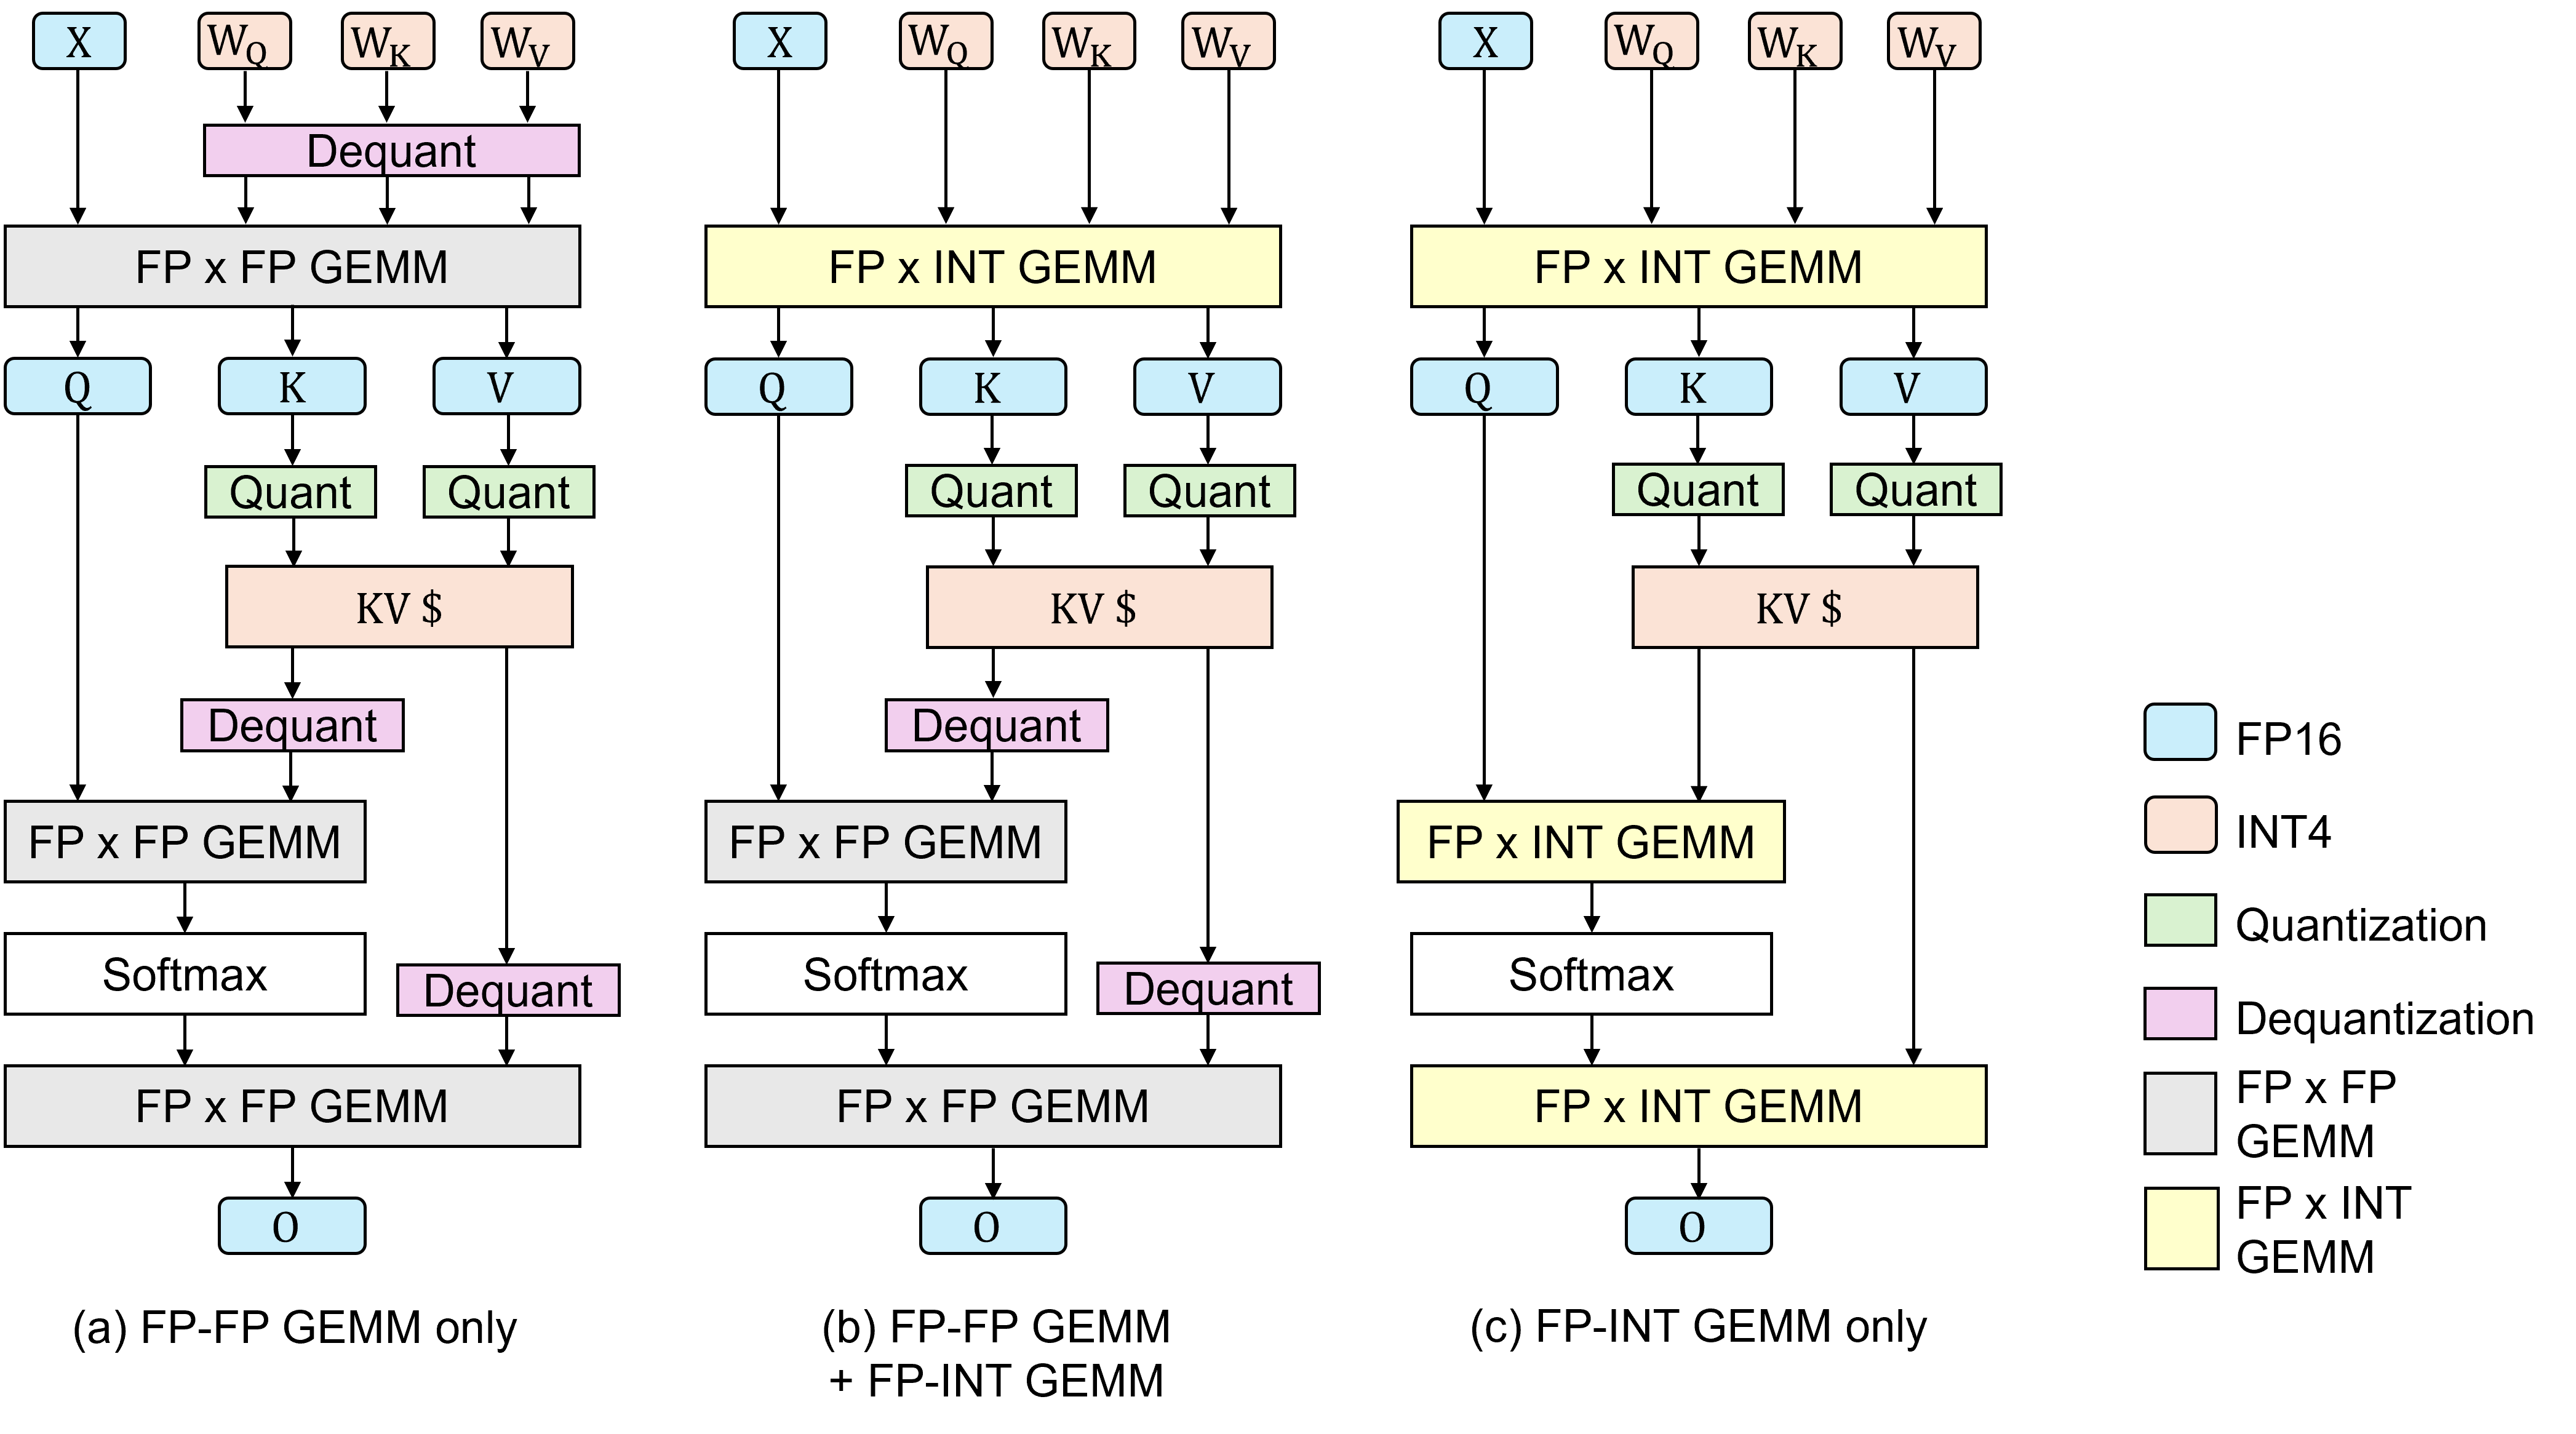
\includegraphics[width=0.92\linewidth]{figures/FIGS_figure1.png}
    \caption{Execution paths for WKV quantized inference: (a) conventional GPU dequantizes INT weight/KV operands before FP GEMM, (b) prior \fpint{} hardware accelerates linear layers but leaves quantized KV attention on the FP path, and (c) our design
  executes both linear and attention GEMMs using native \fpint{} paths.}
    \label{fig:fpint_inference}
\end{figure}

%\begin{figure}[H]
%    \centering
%    \fbox{\parbox{0.92\linewidth}{
%    \centering
%    \vspace{10mm}
%    \textbf{Figure Placeholder: FPxINT inference diagram}\\
%    WKV quantization 한 model의 inference 과정을 쉽게 이해할 수 있도록 간단하게 diagram을 그려준다.\\
%    KV는 dequant 하는 버전하고 KV를 INT로 사용하는 버전하고 같이 그려주자 \\
%    \vspace{10mm}
%    }}
%    \caption{WKV quantized model inference has only FPxINT gemm.}
%    \label{fig:fpint_inference}
%\end{figure}

\subsection{Why Memory Saving Alone is Insufficient}

Quantization의 가장 직접적인 이득은 memory footprint 감소이다.
하지만 serving 환경이 high batch 또는 long sequence로 이동하면 compute demand가 빠르게 증가한다.
Prefill 단계는 긴 prompt를 한 번에 처리하므로 일반적으로 compute-bound 성격이 강하다.
Generation 단계는 token-by-token으로 실행되어 KV cache traffic이 중요해서 memory bound인 경우가 많지만, GQA/MQA/MLA와 같은 구조는 KV head 수 또는 KV representation을 줄여 compute bound 쪽으로 가까워지는 경우가 있어서 computation이 안 중요하다고 할 수 없다. (Figure \ref{fig:bottleneck-analysis})
따라서 최신 LLM에서는 quantization으로 memory traffic을 줄이는 것만으로는 성능 향상이 충분하지 않으며, quantized operand를 dequantization 없이 직접 높은 효율의 연산기로 계산하는 compute path가 필요하다.

\begin{figure}[H]
    \centering
    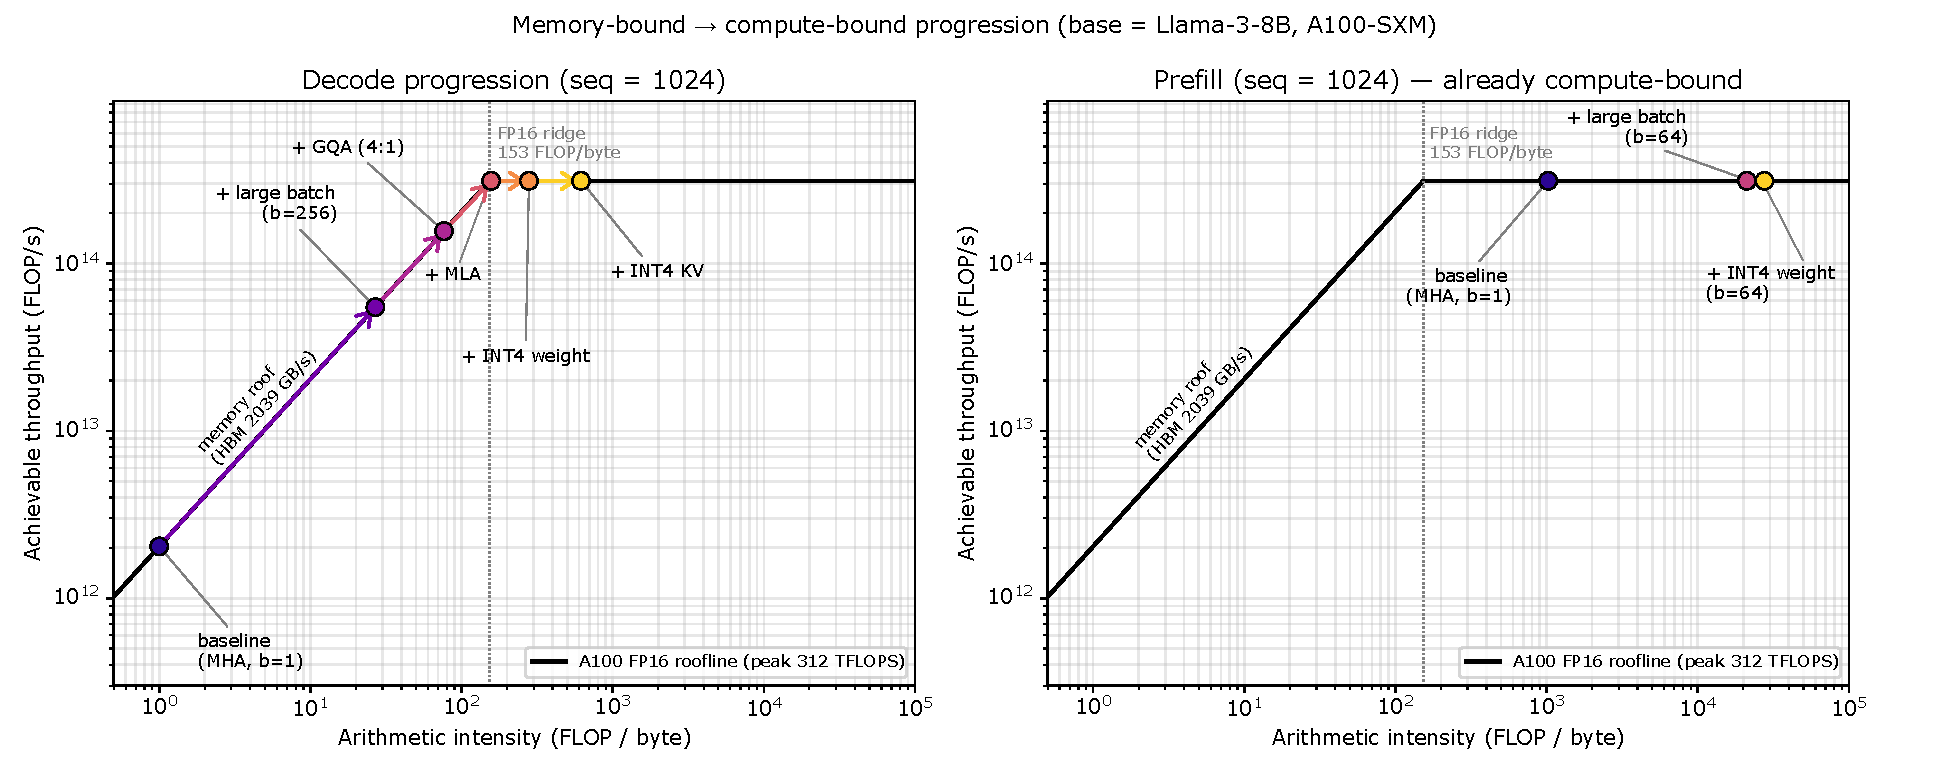
\includegraphics[width=0.92\linewidth]{figures/progression_roofline_refine.pdf}
    \caption{Memory traffic reduction alone becomes insufficient as arithmetic intensity increases.}
    \label{fig:bottleneck-analysis}
\end{figure}

\subsection{Software mpGEMM Optimization and Its Limitation}

소프트웨어 기반 quantized GEMM kernel은 dequantization과 GEMM을 fusion하여 memory movement를 줄이고 Tensor Core utilization을 높인다.
이 접근은 기존 GPU에서 즉시 사용할 수 있다는 장점이 있다.
그러나 INT operand를 FP로 바꾼 뒤 FP Tensor Core로 계산하는 구조는 그대로 유지된다.
즉 latency 관점에서 dequantization을 overlap할 수는 있어도, TOPS와 energy 관점에서 여전히 한계가 분명하다.
energy 관점에서는 dequantization과 FPXFP TCU의 높은 MAC 비용이 남는다.
LLM 같이 대량 serving 하는 system에서는 이제 power delivery가 data center의 bottleneck이 되고 있기 때문에 에너지 효율은 더 이상 무시할 수 있는 factor가 아니다.
TOPS 관점에서는 area cost가 큰 FPxFP TCU를 사용하기 때문에 \fpint{} unit을 썼을 때 추가적으로 얻을 수 있는 throughput을 얻지 못하고 있는 한계가 있다.
latency hiding을 통해서 TCU를 잘 사용할 수 있는 상황에서 TCU가 더 많은 MAC이 있었다면 throughput을 증가시킬 수 있는 상황에서 FPxFP TCU는 \fpint{} unit에 비해 TOPS/mm2이 작기 때문에 성능 향상을 손해보고 있는 것이다. 
FPxINT Gemm unit을 제안한 paper를 보면 FPxFP 연산기에 비해 FPxINT 연산기가 format에 따라서 TOPS/mm2 과 TOPS/W 모두에서 약 2--9배 수준의 이득을 보인다고 보고했다~\cite{figna}. \todo{Comment : 사소하지만 TOPS/mm2 이랑 TOPS/W가 각각 얼마나 더 좋았졌는지를 분리해서 쓰는게 좋을 것 같습니다.}
따라서 high-throughput LLM serving에서는 성능과 에너지 효율성 향상을 위해서는 software 최적화만으로는 한계가 있고 native \fpint{} hardware support가 필요하다.

\subsection{Hardware mpGEMM Accelerator and System-Level Gap}
\label{sec:sys_gap}

기존 mixed-precision hardware 연구는 custom array 또는 lookup-table 기반 unit으로 FP와 INT 사이의 곱셈을 효율적으로 처리한다. 
이들은 array-level에서 높은 TOPS/mm2과 TOPS/W를 보이지만, 실제 LLM inference 전체 성능 향상으로 이어지는 데에는 세 가지 gap이 있다.

\paragraph{Gap 1: \fpint{} Native Attention can not be supported at prefill and generation stage}
기존에는 KV quantization을 generation stage에서의 KV cache를 줄이기 위해서 사용하는 경우가 많았고 일반적인 GPU에서는 FPxFP 연산기 밖에 없기 때문에 prefill에서는 KV cache quantization을 gemm 연산을 가속하는데 사용하지 않고 오히려 후처리 overhead처럼 취급된다. (Figure \ref{fig:prefill_difference}) 하지만 long sequence에서 perfill stage에서 attention에 포함된 연산량이 O(N2)으로 증가하기 때문에 TTFT의 상당 부분을 Attention이 차지하게 된다. (Figure \ref{fig:long_seq_atten_overhead})
즉 prefill에서 KV quantization을 gemm 연산을 가속하는데 활용하는 것이 TTFT를 줄일 수 있는 아주 유망한 방법이다.

문제는 기존 design은 gemm unit의 한계 떄문에 Attention에 있는 gemm은 무시하고 linear layer의 \fpint{} GEMM만 가속하고 있어서 prefill에서 KV quantization을 TTFT를 줄이는데 전혀 활용을 못하고 있고 그로 인해서 long sequence에서 E2E 성능 향상이 매우 제한된다.
\begin{figure}[H]
    \centering
    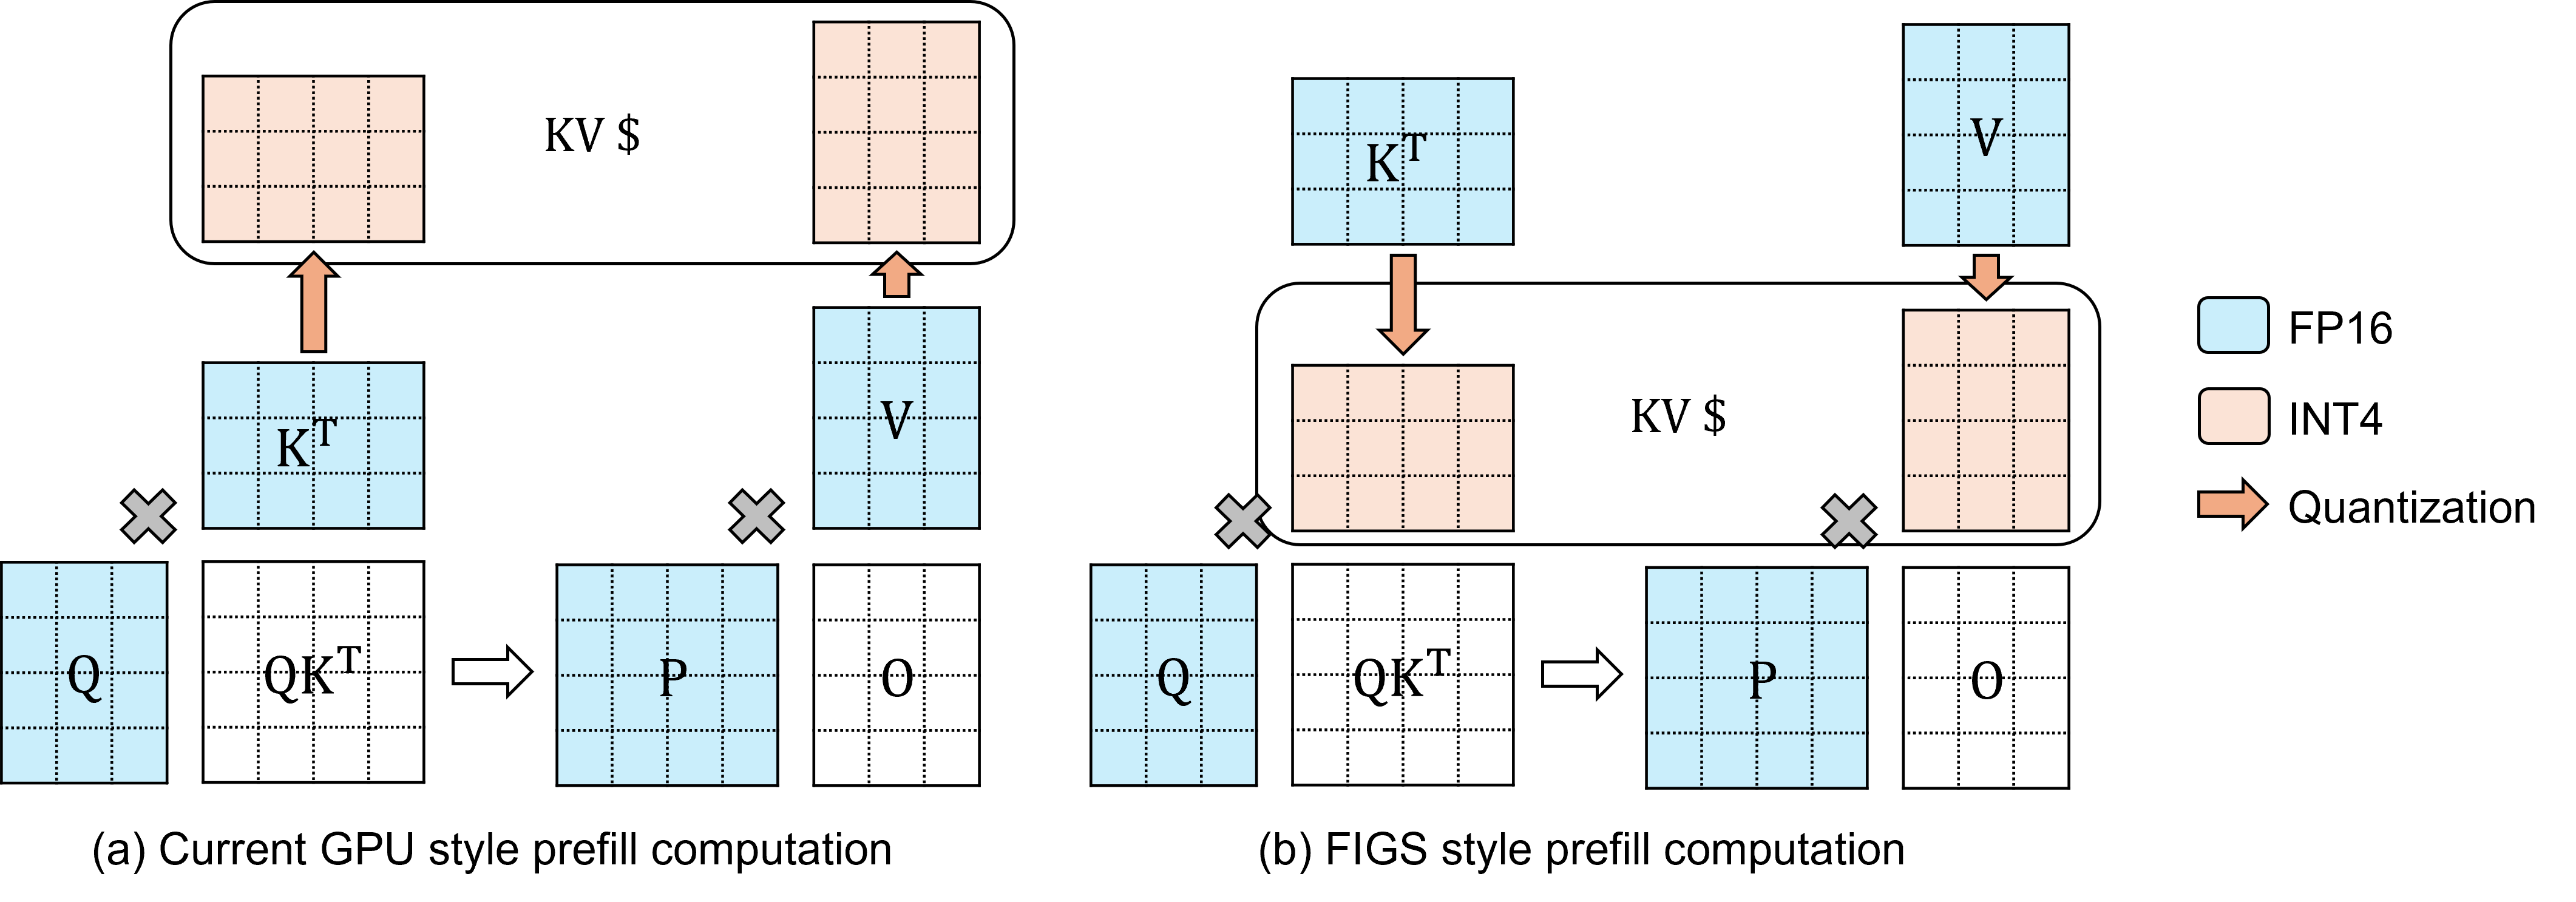
\includegraphics[width=0.92\linewidth]{figures/FIGS_figure_prefill.png}
    \caption{현재 GPU는 prefill 연산을 KV를 FP16으로 연산하지만, Ours는 KV를 INT4로 quantize해서 연산한다.}
    \label{fig:prefill_difference}
\end{figure}

\begin{figure}[H]
    \centering
    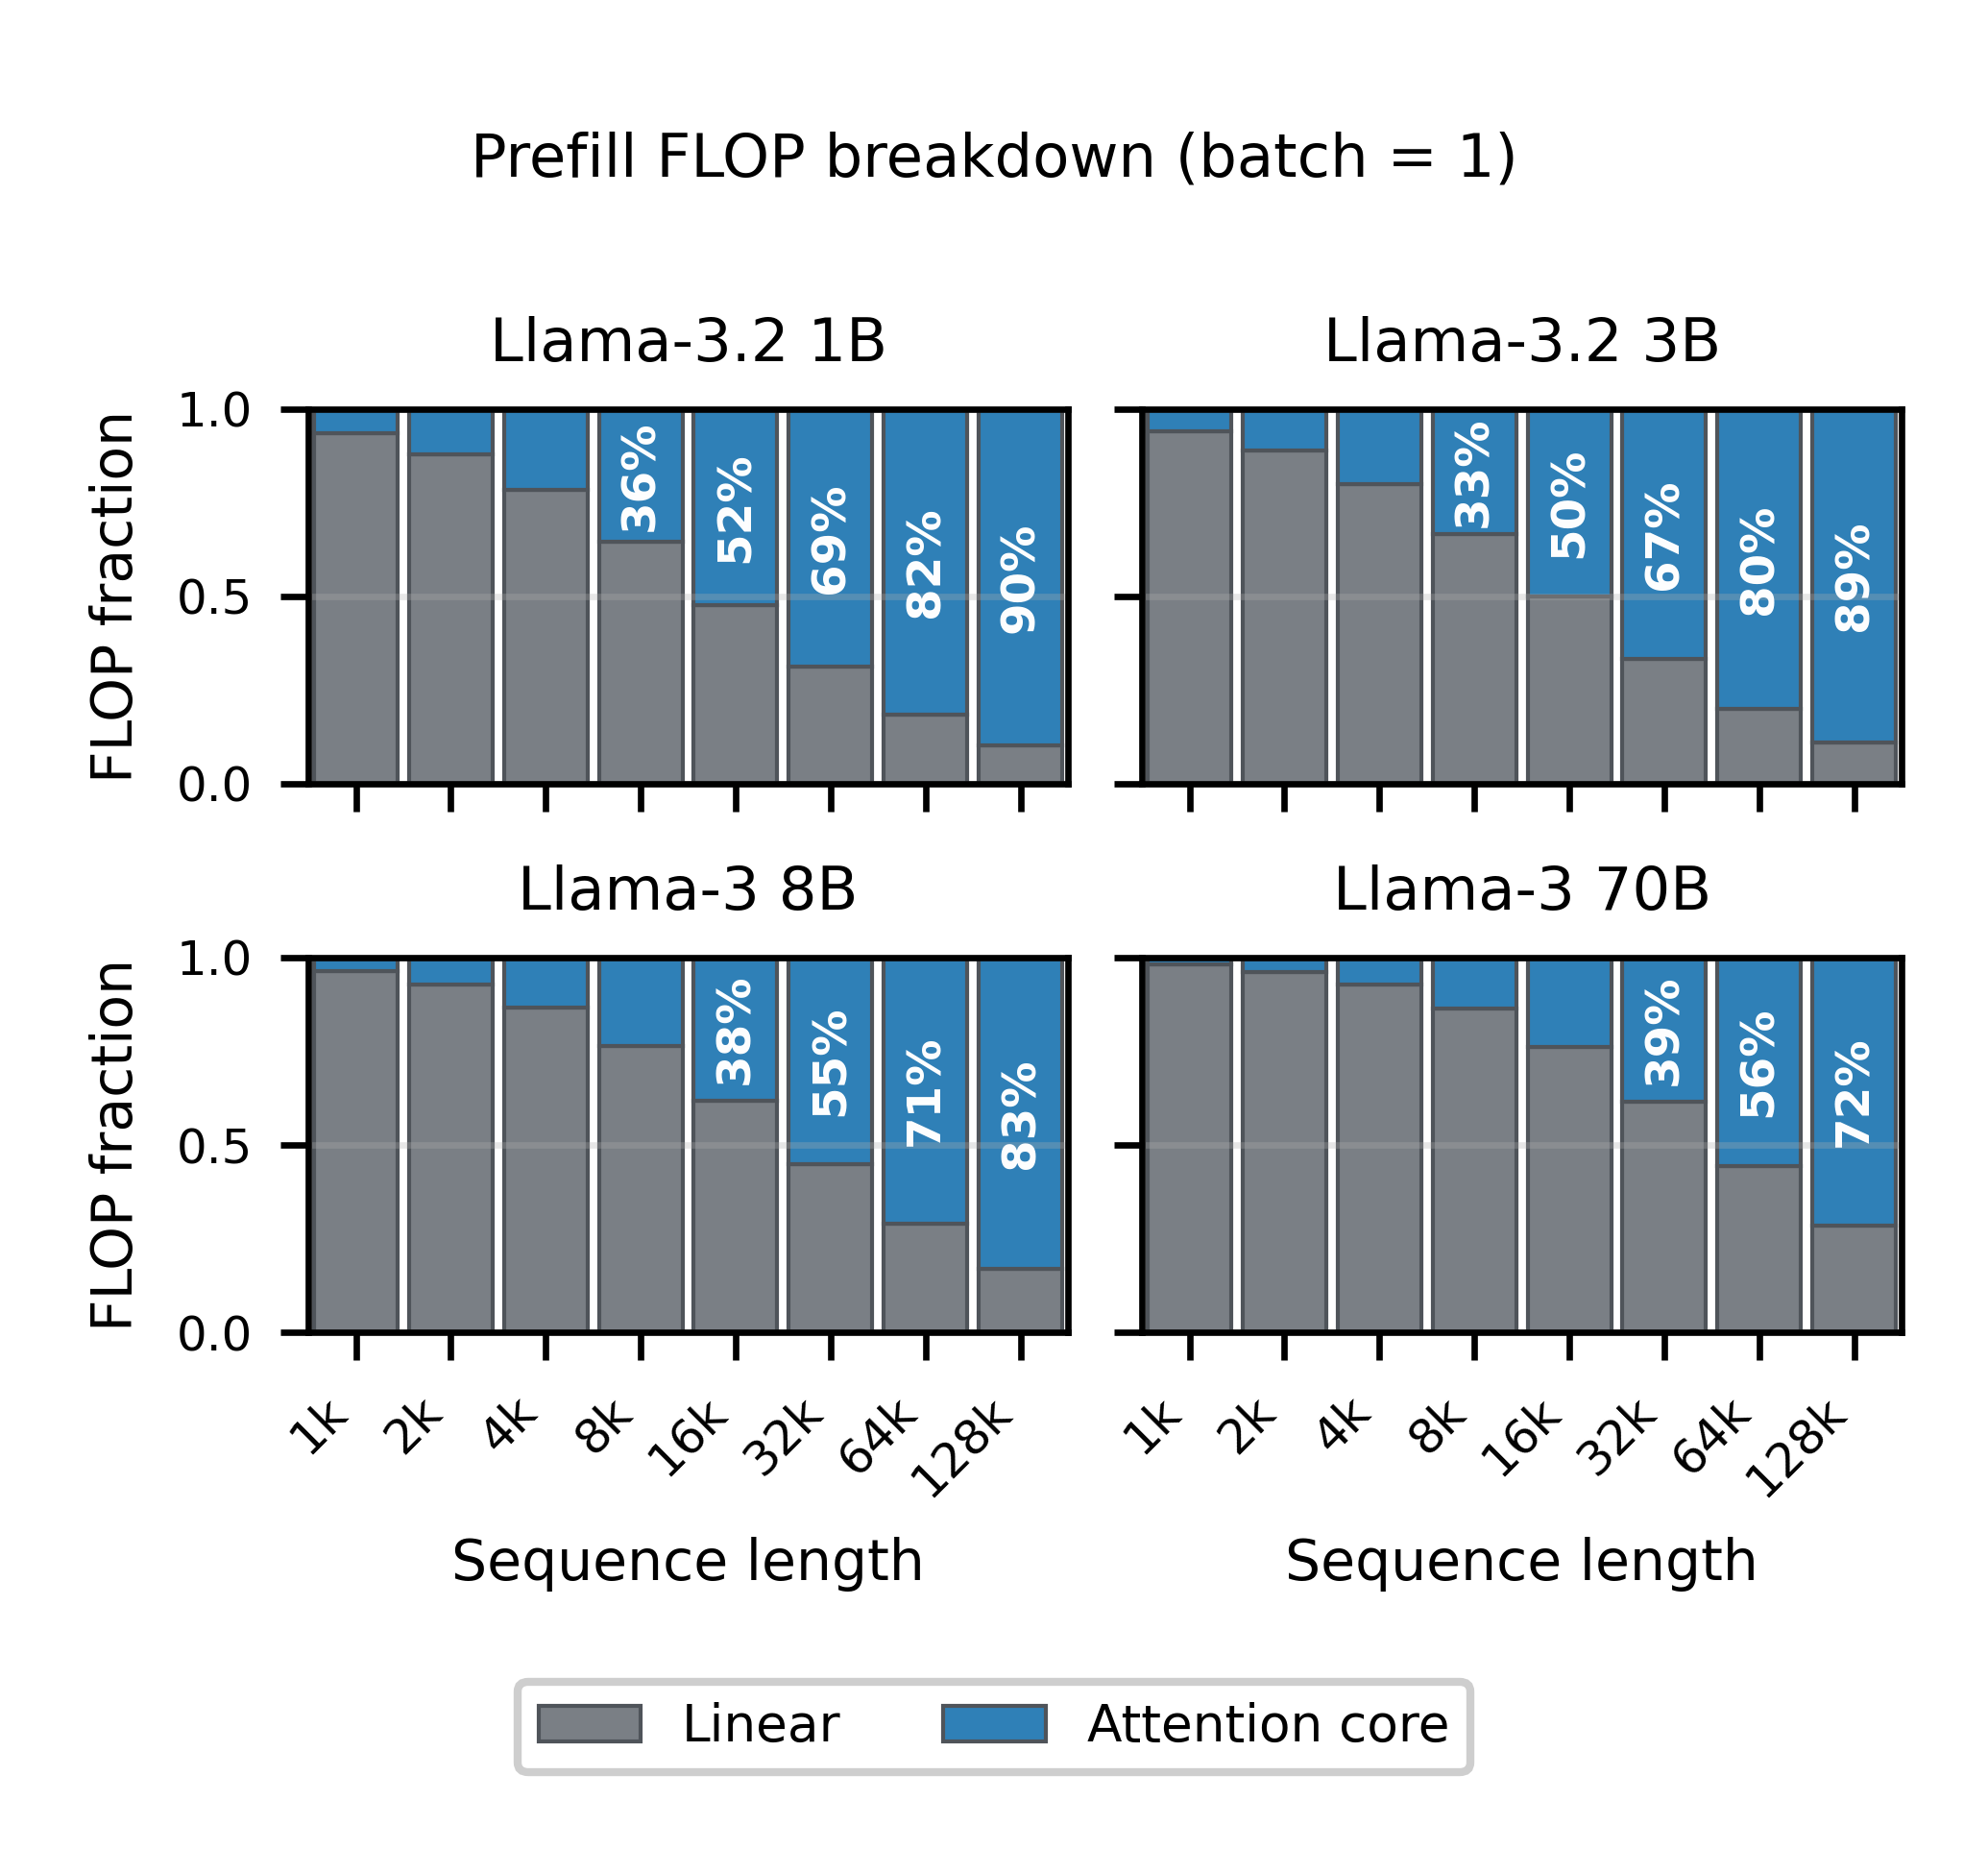
\includegraphics[width=0.92\linewidth]{figures/long_seq_attn_breakdown.png}
    \caption{long sequence에서는 attention 쪽을 가속하는게 중요하다}
    \label{fig:long_seq_atten_overhead}
\end{figure}

기존 work가 FPxINT attention을 지원하지 않는 첫번째 이유는 KV의 quantization 방향이 기존 NPU의 연산 unit에 friendly 하지 않기 때문이다.
%일반적으로 사용되는 quantization framework 중 하나인 SpinQaunt의 경우 generation stage에서 step에 따라 변하는 token 갯수 때문에 Value tensor의 quantization 방향을 항상 head dim으로 size가 고정된 row 방향으로 한다.
일반적으로 사용되는 quantization framework의 Key, Value tensor의 quantization 방향 취합해보면 KV 둘다 token-wise와 head-wise로 고정되어서 사용되는 것이 아니라 framework 마다 방향이 다른 경우가 많다 (Table \ref{tab:kv_quant_granularity})
~\cite{liu2024kivi,hooper2024kvquant,he2024zipcache,yue2024wkvquant,duanmu2024skvq,ashkboos2024quarot,liu2024spinquant}.

\begin{table}[H]
\centering
\caption{Quantization granularity of KV-cache quantization schemes.}
\label{tab:kv_quant_granularity}
\begin{tabular}{p{0.34\linewidth}p{0.34\linewidth}p{0.26\linewidth}}
\toprule
Scheme & K Direction & V Direction \\
\midrule
KIVI / KVQuant / ZipCache & channel-wise & token-wise \\
WKVQuant / SKVQ & token-wise & token-wise \\
QuaRot / SpinQuant & token-wise or channel-wise & token-wise \\
\bottomrule
\end{tabular}
\end{table}

K의 경우 channel-wise 인 경우, V의 경우 token-wise의 경우 gemm 연산을 할 때 reduction dimension 쪽으로 전부 다른 scale factor를 가지기 때문에 기존 NPU의 GEMM 연산기로 처리하려면 INT reduction 연산기를 쓰지 못하고 INT 곱셈 한번하고 그 결과를 FP로 deqaunt하는 overhead에 추가로 FP reduction을 해야해서 기존의 효율성이 사라진다 (Figure \ref{fig:quant_row_dir_overhead}).

\begin{figure}[H]
    \centering
    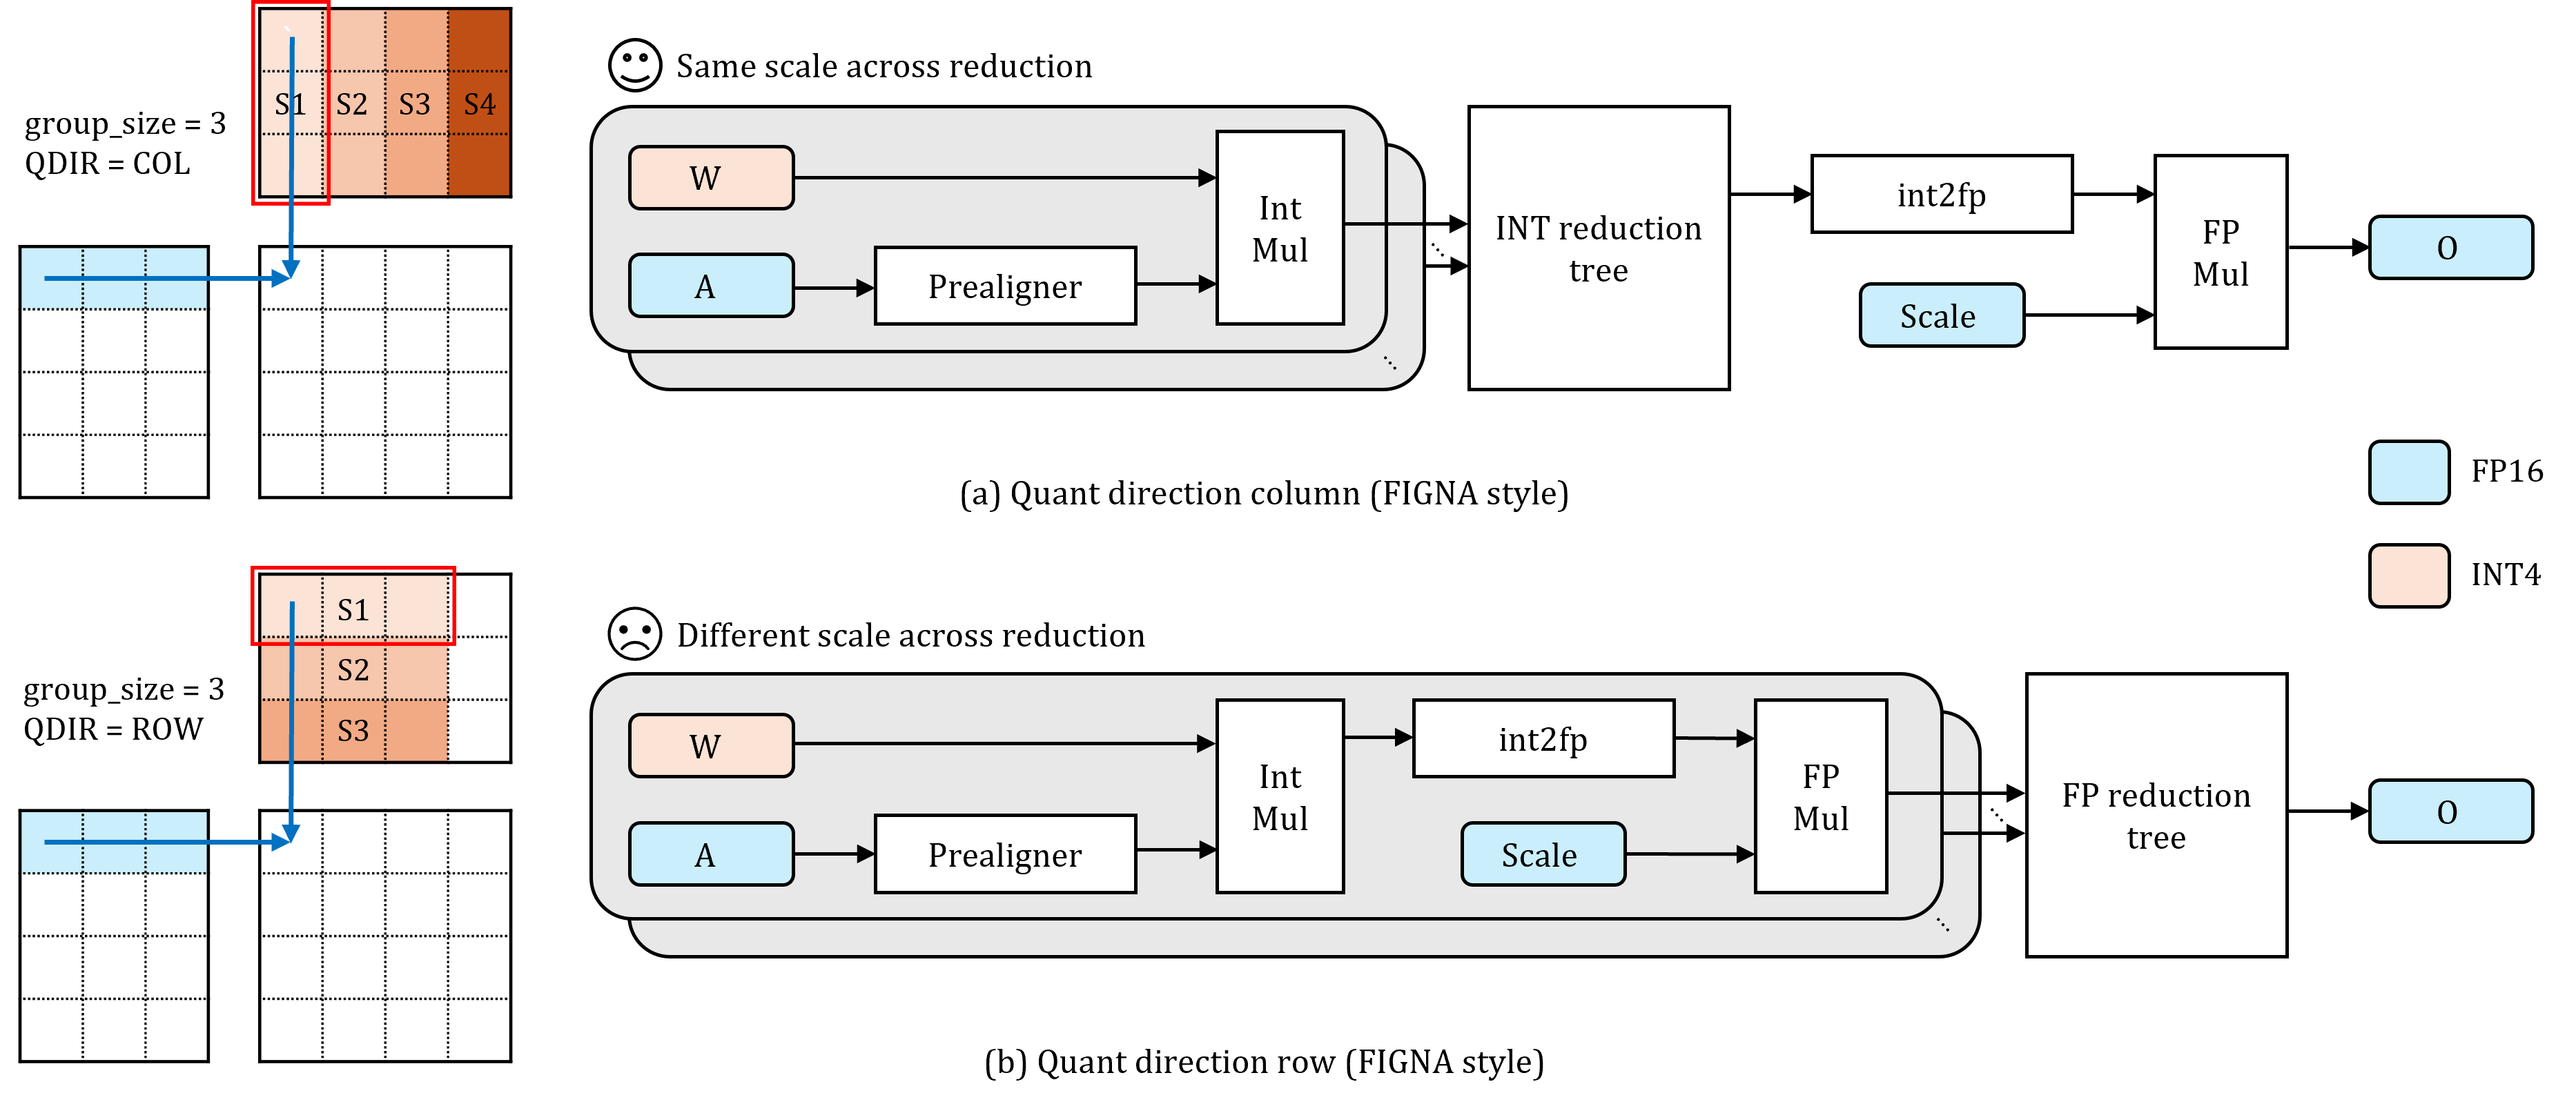
\includegraphics[width=0.92\linewidth]{figures/FIGS_figure4_new2.png}
    \caption{row 방향 quantization을 할때 기존 NPU 구조로 하면 overhead가 생긴다}
    \label{fig:quant_row_dir_overhead}
\end{figure}

%\begin{figure}[H]
%    \centering
%    \fbox{\parbox{0.92\linewidth}{
%    \centering
%    \vspace{12mm}
%    \textbf{Figure Placeholder: quant direction challenge}\\
%    row 방향 quantization을 할때 기존 NPU 구조로 하면 어디서 overhead가 생기는지 그림으로 보여주자. 간단한 실험을 해서 얼마나 overhead가 생기는지 숫자로 넣어주자.\\
%    \vspace{12mm}
%    }}
%    \caption{Overview of the proposed hardware/software system.}
%    \label{fig:quant_row_dir_overhead}
%\end{figure}

%두번째는 weight는 compile time constant이기 때문에 weight에 전처리를 해서 효율적으로 연산하는 경우가 많은데 KV의 경우 dynamic하게 생성되기 때문에 전처리가 불가해 전처리 overhead가 생기기 때문이다. 예를 들어 FIGLUT과 LUT-TC는 LUT의 size를 줄이기 위해서 weight에 preprocess를 해서 대칭화 시키는 전처리를 한다.
%\todo{DISCUSS : 실제 overhead가 어느정도 인지 숫자가 필요하다. 근데 overhead가 작을 가능성이 커서 실제로 작은 경우 그냥 dynamic challenge는 빼는 것이 좋을듯하다.}

\paragraph{Gap 2: A Larger MXU Alone Does Not Guarantee Performance Gains}
%LLM은 prefill만 잘하면 되는게 아니다. generation stage도 workload에 따라 latency를 prefill 보다 더 크게 소모할 수 있다.
%기존 FPxINT hardware는 generation stage에서의 가속을 크게 고려하지 않는다.
\fpint{} unit의 높은 TOPS/mm2를 활용해서 같은 면적에 더 큰 MXU를 넣은 것만으로는 system level에서 실제 성능 향상을 보장할 수 없다.
%generation stage에서도 속도 향상을 얻으려면 같은 면적에 더 많은 MAC을 넣었을 때도 array util을 크게 유지해야한다.
TOPS/mm2을 이용해서 더 높은 TOPS를 얻기 위해서는 MXU의 utilization을 MAC의 개수가 많아졌을 때도 계속 높게 유지해야하는데 기존의 NPU들은 array level의 성능 향상에 집중하고 실제 system에서의 utilization을 높게 유지하는 연구는 깊게 하지 않았다.

MXU의 util을 높게 유지하기 위해서는 크게 두가지를 해야한다. 첫번째는 커진 MXU size에 맞게 memory subsystem의 peak bandwidth도 scaling 해야한다. 두번째는 scale된 memory subsystem을 low-latency and bursty하게 잘 사용해야한다.
%HBM 에서 on chip memory로 가는 부분과 on chip memory에서 gemm unit으로 가는 network의 bandwidth를 크게 scaling 해야한다.

memory subsystem의 bandwidth를 scaling하는 것은 생각보다 쉽지 않는데, 그 이유는 일반 GPU-style memory hierarchy에서는 shared memory, cache, register file등 memory subsystem 전반에 걸쳐서 general-purpose 접근을 지원해야 하므로 xbar를 빈번히 사용하기 때문이다. ~\cite{jin2024uncovering, tine2021vortex}.
그 결과 FPxFP MXU를 \fpint{} MXU로 바꾸면서 memory subsystem을 같이 scaling할 때 xbar를 사용하는 architecture를 유지한채 naive하게 scaling하면 xbar의 O(N2)으로 커지는 cost 때문에 TOPS/mm2 향상이 system level에서 보면 이득이 거의 없거나 심하면 오히려 TOPS/mm2이 떨어진다 (Figure \ref{fig:xbar_overhead}).

memory subsystem의 bandwidth를 scaling 할때 사용하는 방식 중 일반적인 것은 bank의 개수를 늘리고 bank를 접근할 때 interleaving address scheme을 사용하는 것이다. 문제는 이 경우에 DMA를 구현할 때 full bandwidth를 사용하게 하는 것은 생각보다 쉽지 않다. 먼저 burst를 할 때 보내는 request는 한번에 가져오는 data가 bank의 경계를 넘어서지 않도록 하는 constraint가 지켜져야한다. 또한 misaligned access가 있으면 이를 지원하기 위해서 barrel shifter가 필요한데 문제는 DMA의 data width를 매우 크게 scaling한 상황에서 barrel shifter도 같이 커지기 때문에 1 cycle만에 misaligned access를 처리하려면 area, power, timing 전부 큰 overhead가 생긴다. %\todo{barrel shifter overhead 측정해보자}

결론적으로 xbar cost에 의해서 bandwidth를 증가시키는 것 자체가 쉬운 일이 아니고 만약 되더라도 bandwidth를 제대로 활용하기 위해서는 DMA에서 매 cycle 생성되는 request가 bank 간의 경계를 넘지 않도록 해야하고 misaligned access를 피해야하는 constraint를 지키면서 burst를 해야된다는 어려움이 있다.
%FPxFP의 경우 면적 cost가 크기 때문에 FPxINT에 비해 TOPS가 크지 않아서 memory subsystem의 bandwidth를 증가시킬 때 기존의 xbar를 사용하는 구조를 그대로 유지하면서 scaling해도 감당이 된다. \todo{감당이 되는거 맞나?}
%이 때 FPxINT로 가면 면적 효율이 좋아서 FPxFP에 비해 FP16의 경우 약 4배정도의 MAC을 더 넣을 수 있고 이걸 실제 generation stage에서 속도 향상으로 가져오기 위해 scaling해야하는 memory subsystem의 bandwidth가 비례해서 4배정도로 커진다.
%결국 FPxFP unit을 쓸 때 보다 FPxINT unit을 쓸 때 generation stage에서의 성능 향상을 위해 memory subsystem scaling을 해야하는 난이도가 급격히 상승한다.
%문제는 xbar의 경우 O(N2)으로 복잡도가 증가해서 FPxFP MXU를 \fpint{} MXU로 바꿀 때 xbar를 그대로 사용하면서 memory subsystem을 scaling하면 감당이 안되서 TOPS/mm2 향상이 생각만큼 안 올라온다 (Figure \ref{fig:xbar_overhead}).
%따라서 array를 크게 만드는 것만으로는 generation stage에서의 system level performance 이득을 얻기에 충분하지 않으며, array를 지속적으로 feed할 수 있는 memory system을 적은 overhead로 scaling하는 것이 중요하다.
%\todo{figure 5 실험에서 L/D/A 설명, figure 5 주석에 energy cost라는 말이 있는데 이거 실험은 없다.}

% ---------------------------------------------------------------------------
% V1
% ---------------------------------------------------------------------------
%Array의 MAC 개수를 늘리면 요구되는 operand bandwidth도 증가한다.
%일반 GPU-style memory hierarchy에서는 shared memory, cache, register file, interconnect가 general-purpose 접근을 지원해야 하므로 xbar를 사용한다. ~\cite{jin2024uncovering, tine2021vortex}.
%port data width와 bank 수 증가가 local memory와 register를 연결하는 xbar, cache system에서 multi bank를 연결하는 xbar 등이 O(N2)으로 커져서 area, timing, routing overhead로 이어진다.
%GPU의 tensor core의 경우 tensor core (TCU)가 커졌을 때 register pressure가 상당히 커진다. tensor core는 register file에서 data를 가져오는데 TCU가 커지면 한번에 접근해야하는 register의 갯수가 비례해서 증가한다. register를 TCU만 쓰는게 아니기 때문에 register pressure에 의해 load/store 명령어 증가와 cache miss 증가로 이어져서 성능 하락이 심하게 온다.
%register file 갯수를 늘리는 것은 쉬운 일이 아닌게 register와 shared memory, ALU 사이에 xbar가 있기 떄문에 overhead가 커진다. (Figure \ref{fig:xbar_overhead})
%따라서 array를 크게 만드는 것만으로는 충분하지 않으며, array를 지속적으로 feed할 수 있는 memory system을 적은 overhead로 scaling하는 것이 중요하다.
\begin{figure}[H]
    \centering
    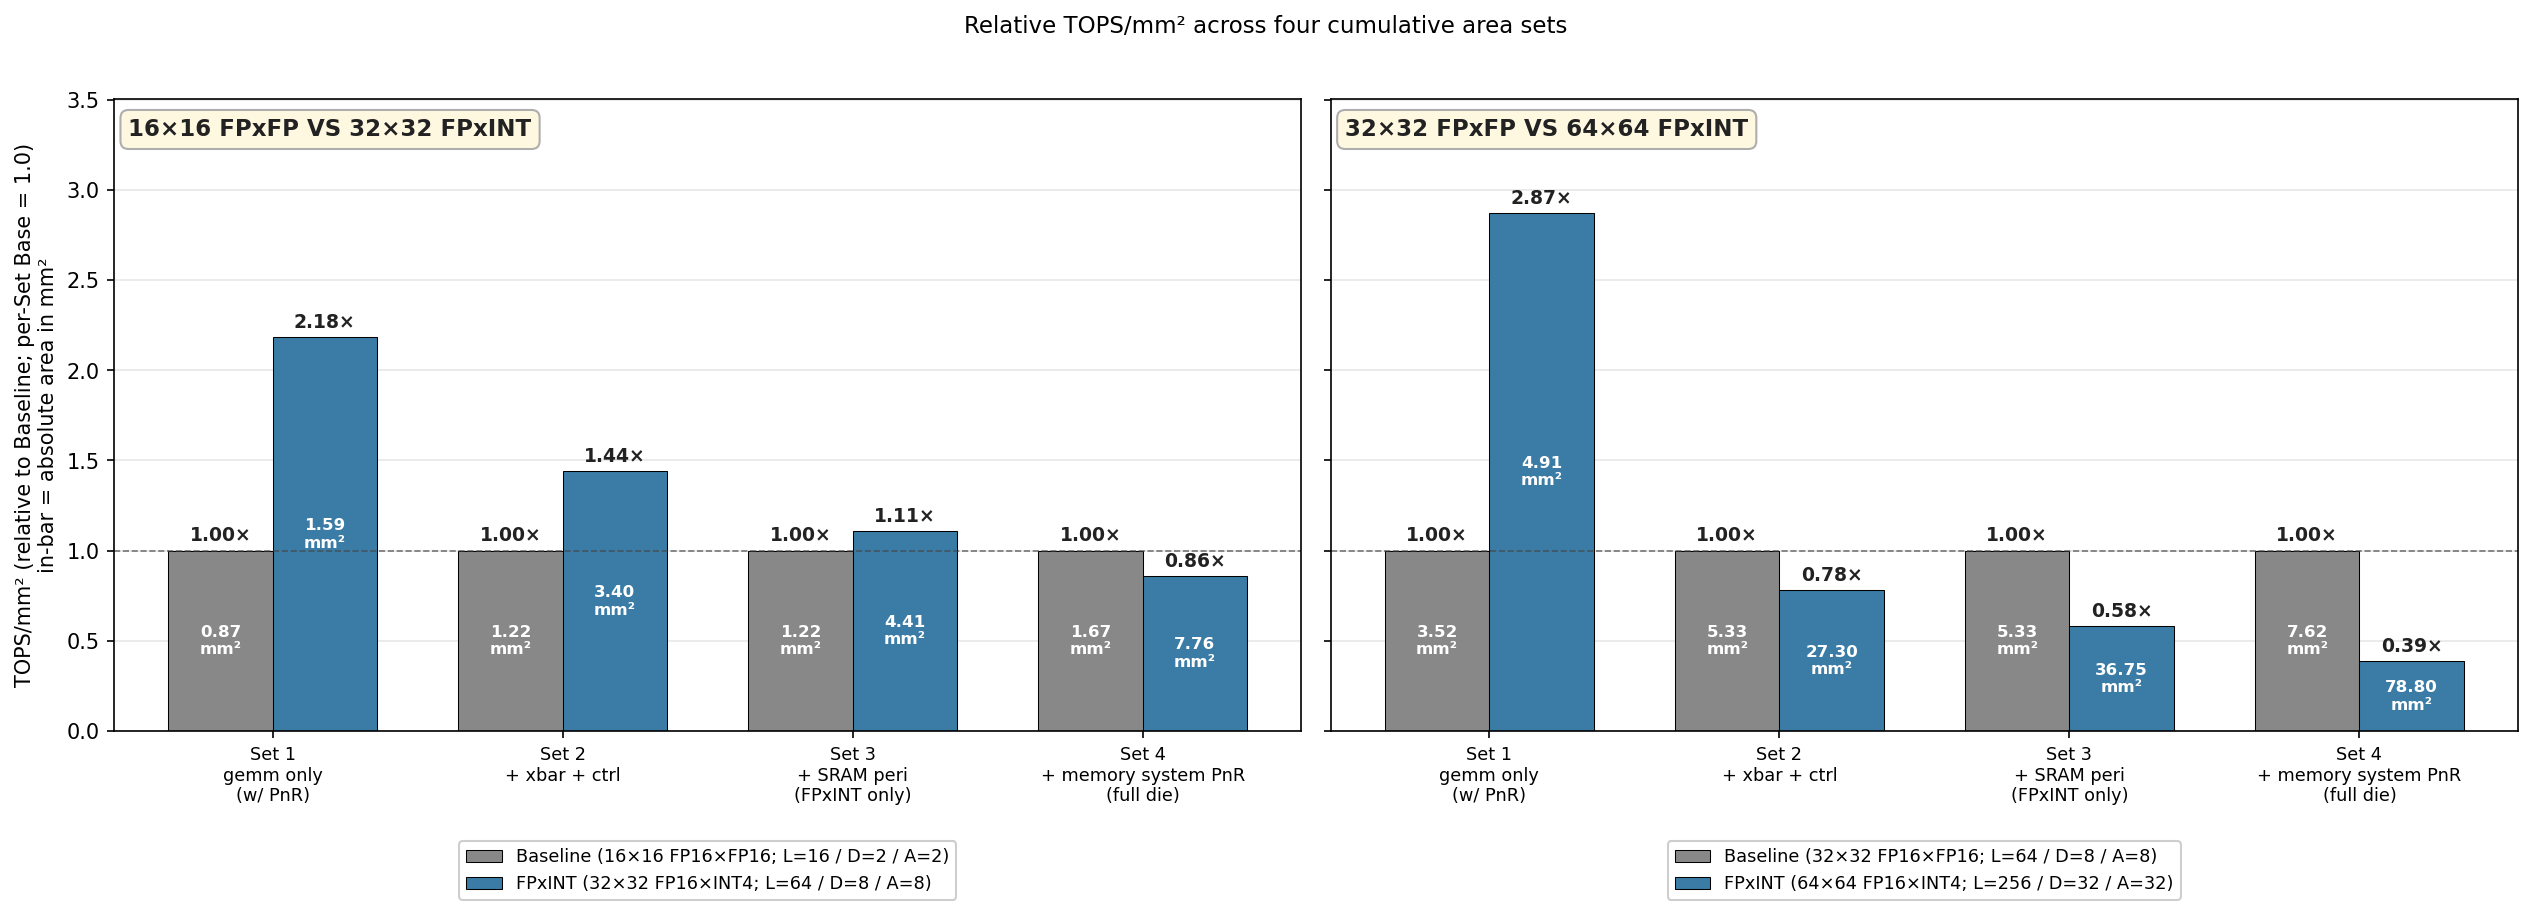
\includegraphics[width=0.92\linewidth]{figures/xbar_overhead.png}
    \caption{Relative TOPS/mm² of FPxFP vs FPxINT GEMM arrays with progressively included memory-system area overheads. Bars are normalized to the FPxFP baseline for each set, with absolute area shown in-bar. GEMM area includes its own   
  PnR; Set 4 includes memory system PnR. CAP-intrinsic SRAM area is excluded, while SRAM peripheral overhead is charged only to FPxINT. L/D/A are LMEM banks/requests, DCACHE banks/requests/ports, and AXI input ports, set by L=$N^2$/16,
  D=A=max(1,$N^2$/128).}
    \label{fig:xbar_overhead}
\end{figure}

%\paragraph{Gap 3: Lack of E2E system}
%실제 LLM inference는 GEMM만으로 구성되지 않는다.
%LayerNorm, residual add, RoPE, softmax, sampling, memory allocation, kernel scheduling이 함께 동작해야 한다.
%hardware뿐 아니라 programming model, runtime, kernel, frontend와의 integration 등 실제 LLM을 E2E로 돌리려면 많은 component가 필요하다.
%기존 accelerator 연구가 isolated GEMM 또는 simplified simulator에 머무르면, 실제 model을 end-to-end로 실행할 때 발생하는 실제 system bottleneck을 관찰하기 어렵다.
%예를 들어 RoCC 형태로 가속기의 instruction을 많이 확장하는데 GPU의 경우 각 warp가 느리기 때문에 RoCC style로 연산을 하면 그게 bottleneck이 된다.(?)
%\todo{DISCUSS : 이게 문제라는 좀 더 명확한 근거 data가 있으면 좋을듯 ; '기존 하드웨어 연구의 한계' 파트에 썼던거 다시 써도 좋을 듯 하다. (예를 들어 LUT TC의 경우 array level TOPS/mm2 improvement가 array level에서는 18배인데 E2E 이득을 보면 2.9배로 준다.)}
%open-source 없는데 우리는 했다.

\section{Design Overview}

\begin{figure}[H]
    \centering
    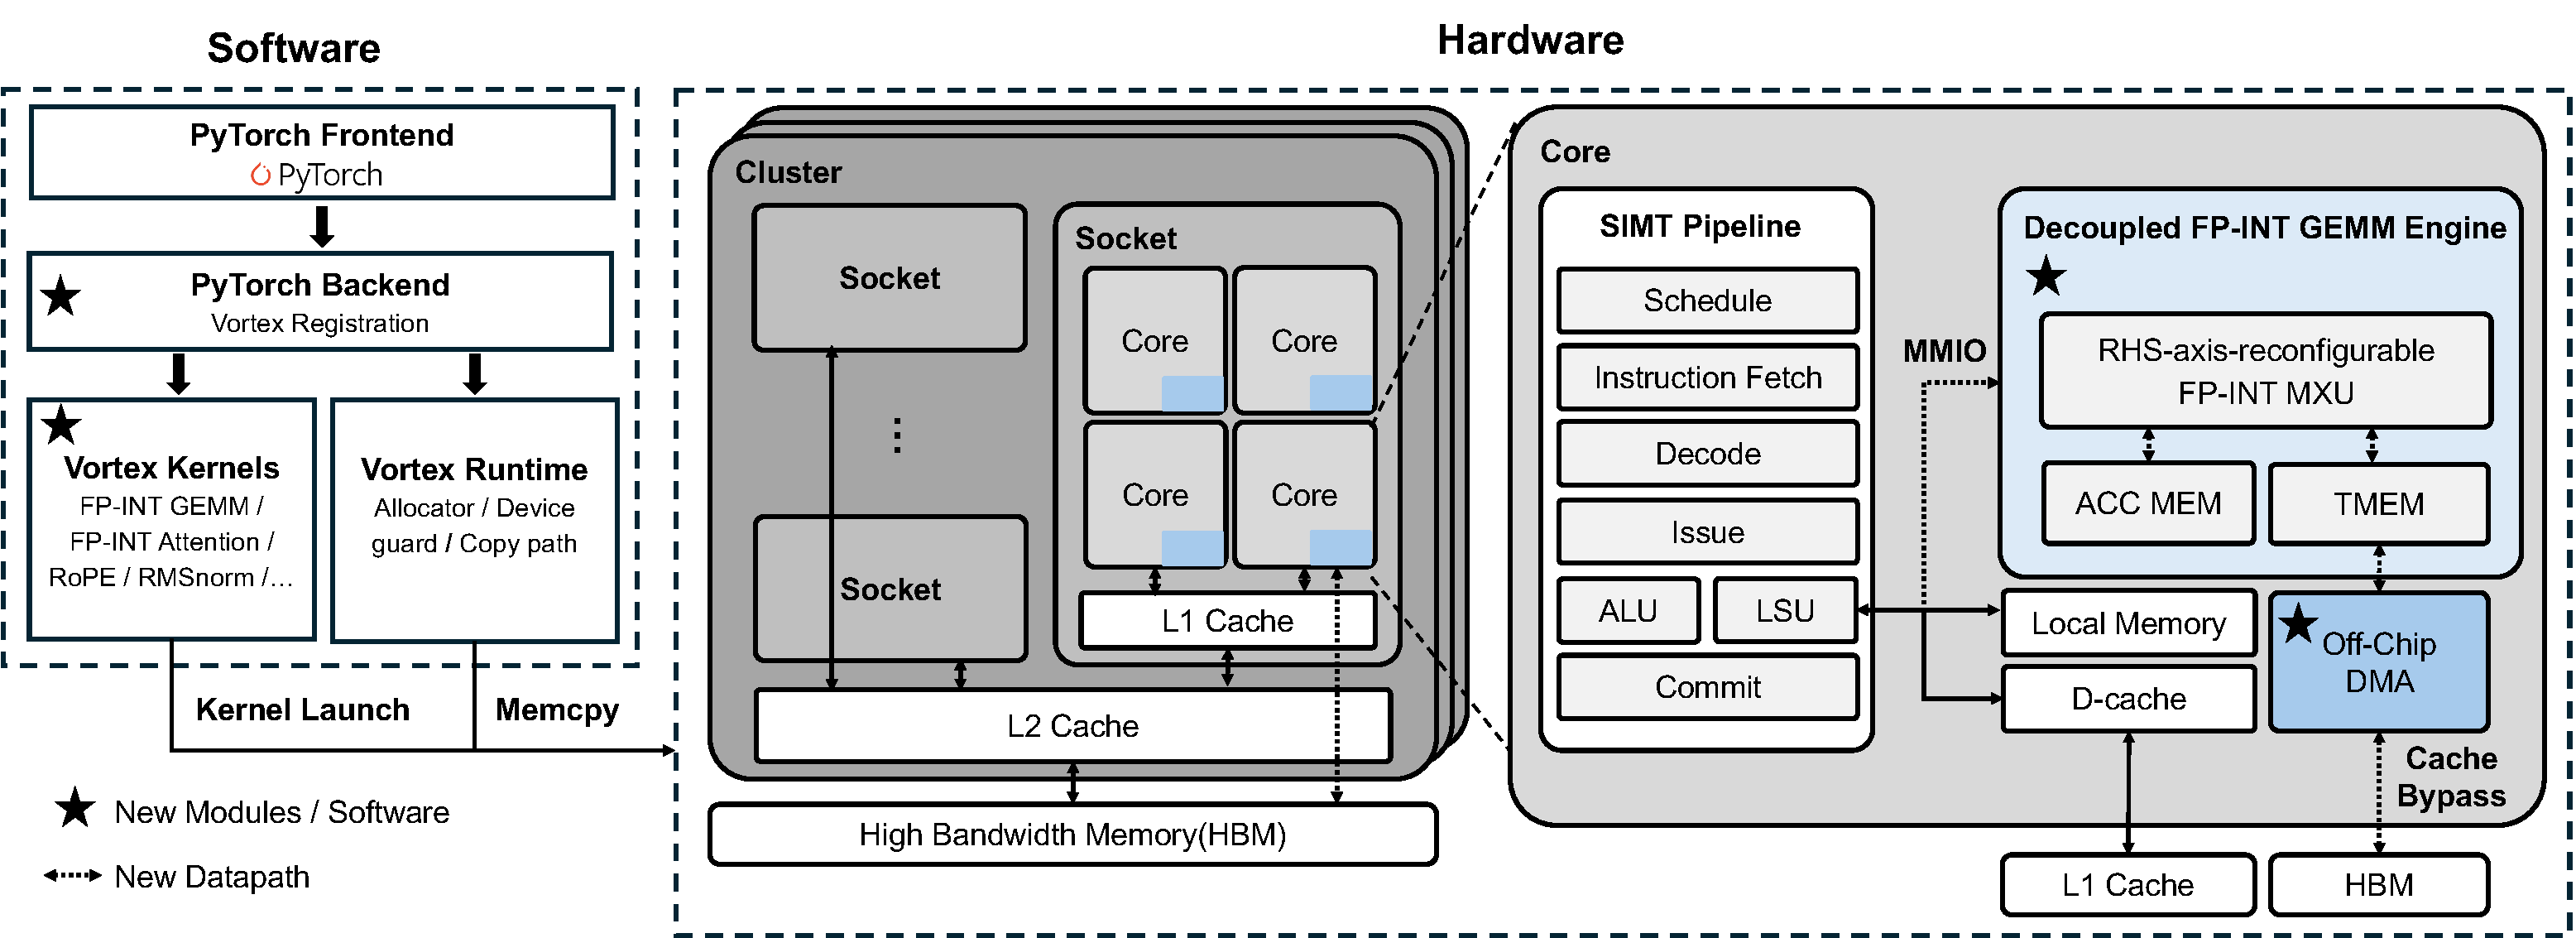
\includegraphics[width=0.92\linewidth]{figures/fig7.pdf}
    \caption{Overview of the proposed hardware/software system.}
    \label{fig:overview}
\end{figure}

\ours{}는 open-source GPGPU인 Vortex를 WKV quantized model을 가속하기 위해 \fpint{} gemm engine과 이를 최대 utilization으로 사용하기 위한 low cost memory subsystem과 software stack을 포함하는 system이다. \todo{위 그림이 그려지면 이거에 대한 설명 필요.}
설계한 system이 E2E에서 효과적으로 가속하기 위해서 여러 decision을 내렸다. 

\paragraph{Vortex의 SIMT pipeline은 유지한다}
LLM에는 gemm 이외에도 다양한 vector 연산이 존재한다. Vector 연산이 연산량이 적다해도 CPU로 fallback하면 overhead가 매우 크기 때문에 programmablity와 generality를 위해서 SIMT pipeline은 유지한다.

\paragraph{\fpint{} gemm engine은 RHS의 quantization direction과 load direction의 모든 조합을 support 하도록 design 해야한다}
\wkv{} quantized model에서 반복적으로 등장하는 \fpint{} GEMM은 RHS matrix의 quantization direction과 transposed된 여부가 다양하다. QK$^T$에서는 RHS가 transposed되어서 연산되어야하고 그외의 PV와 linear projection, FFN에서는 non-transpoed이다. Quantization direction은 Table \ref{tab:kv_quant_granularity}에서 볼 수 있듯이 KV의 quantization이 token-wise 와 channel-wise 둘 다 존재한다. 즉 \fpint{} gemm engine이 WKV quantized model을 fully 가속하려면 4가지의 연산방식을 reconfigurable하게 support할 수 있어야 한다. 

\paragraph{gemm engine을 SIMT에서 decouple 시키고 gemm을 위한 독립적인 tensor memory와 acc memory를 사용한다}
가장 일반적으로 언급되는 TCU의 가장 큰 문제는 register pressure이다. 이 문제는 TCU의 크기가 커질수록 더 심해진다. \fpint{} gemm engine의 경우 높은 TOPS/mm2을 활용해서 큰 MXU를 사용할 수 있기 때문에 SIMT core에 coupling 시켜두면 register pressure에 의해 utilization을 높게 유지할 수 없다. 이를 해결하기 위해서 \ours{}는 gemm engine을 SIMT core에서 decouple 시킨다. gemm engine과 communication할 memory를 GPU의 shared memory를 사용하면 shared memory가 xbar 기반으로 연결되어 있기 때문에 bandwidth scaling이 쉽지 않고 SIMT core의 load, store 명령어와의 conflict에 의해 gemm engine의 utilization이 떨어질 수 있기 때문에 독립적인 shared memory의 capacity를 일부 tensor memory로 나눠서 독립적인 memory space를 구성한다. 또한 quantized model 특성상 input과 weight 보다 dequantization 때문에 psum의 bitwidth가 더 크다. Gemm engine에 acc memory를 따로 두면 input, weight에 사용할 bandwidth를 소모하지 않아도 되고 conflict free를 dataflow level에서 보장할 수 있기 때문에 gemm engine 내부에서 word-wise ping-pong scheme을 사용해서 single port sram으로 back pressure signal 없이 full throughput으로 gemm 연산을 진행할 수 있다.

\paragraph{GEMM command stream은 software queue가 아니라 hardware micro-op FSM이 생성한다}
큰 \fpint{} MXU는 operand bandwidth뿐 아니라 command bandwidth도 요구한다. 초기 설계는 kernel이 bit manipulation으로 tile-level CMD를 생성하고 store 명령으로 CMD queue에 enqueue하면, hardware가 이를 decode하는 방식이었다. 그러나 본 논문의 Vortex 기반 GPU에서는 warp 하나가 만드는 scalar command stream이 충분히 빠르지 않아서, command packing과 queue store가 GEMM launch path의 bottleneck이 되었다. \todo{Comment : 이게 Vortex에서만 못하는 건가요 아니면 GPU에서도 못 하는건가요? GPU에서도 못 하는걸 판단할 근거가 없으면 GPU라고 써도 되는지 모르겠어요.} \ours{}는 kernel이 MMIO register에 matrix shape, stride, tensor/accumulator base address, qdir, load direction, scale/zero-point metadata를 programming하고 doorbell로 request를 제출하는 구조를 사용한다. Request slot allocation이 성공하면 gemm engine 내부의 micro-op generation FSM이 descriptor를 DMA, RHS load, MXU step, accumulator update, completion signaling으로 확장한다. 즉 SIMT pipeline은 compact descriptor setup과 synchronization만 담당하고, 반복적인 GEMM micro-op stream은 hardware sequencer가 생성한다.

\paragraph{복잡한 xbar를 쓰면서 memory subsystem을 scaling하지 않고 simple한 interconnect fabric을 사용해서 low cost로 scaling하고 추가된 constraint는 software stack에서 handling한다}
memory subsystem을 scaling할 때 xbar를 가지고 있는 component를 그대로 scaling 하면 오히려 TOPS/mm2이 안 좋아진다. 이를 해결하기 위해서 \ours{}는 HBM의 Pseudo channels, Tensor memory bank, gemm engine의 lane 사이를 xbar 없이 연결한다. 이때 tensor traffic은 cache hierarchy를 거치지 않는 별도의 DMA path로 이동한다. 이는 cache/local-memory interconnect를 \fpint{} operand bandwidth에 맞춰 확장할 때 발생하는 xbar cost를 피하기 위한 선택이다. Non-coherent bypass path가 만드는 correctness 문제는 arbitrary sharing을 지원하는 hardware protocol로 해결하지 않고, GEMM kernel의 phase-based buffer ownership과 explicit synchronization으로 처리한다. source와 destination component의 개수가 같으면 1:1 connection을 하고 다르면 simply interleaved connection을 사용해서 연결한다. 이 때 부작용으로 xbar를 사용하지 않았기 때문에 data 이동의 constraint가 생긴다. 예를 들어 HBM address X에 있는 data를 TMEM address Y로 옮길 수 없는 경우가 생길 수 있다. gemm의 경우 규칙적인 dataflow 덕분에 이런 constraint가 매우 간단해져서 compiler/runtime/kernel design 등 software stack에서 큰 노력 없이 constraint을 met할 수 있다. 결과적으로 total area가 약 3\% 증가하는 정도로 memory bandwidth를 8배 scaling 할 수 있었다. \todo{Comment : 이 hardware overhead가 정확히 무엇인지 써줘야 할 것 같아요.}
%HBM channel과 on-chip tensor memory bank를 xbar를 사용하지 않고 단순한 PC 와 bank 사이의 1:1 path로 연결하여 interconnect overhead를 줄인다. 이 제약은 compiler/runtime/kernel 설계에서 address alignment와 layout rule로 처리한다. 또한 base address에 대한 constraint를 만족 시키기 위해 HBM에 주소를 allocation할 때 base address가 특정 숫자에 align 시키는 제약을 줄 수 있도록 vortex runtime을 확장한다.

%\paragraph{Usability를 위해서 PyTorch Integration을 구현한다}
%PyTorch integration은 PrivateUse1 backend를 통해 quantized operator를 Vortex kernel로 dispatch한다.
%Frontend는 \wkv{} quantized tensor와 metadata를 유지하고, backend는 operator pattern에 따라 native \fpint{} linear, QK$^T$, PV kernel을 선택한다.
%이 stack 덕분에 \ours{}는 단순 GEMM microbenchmark가 아니라 실제 LLM inference graph 안에서 memory system, runtime layout, native attention support가 함께 작동하는지를 평가할 수 있다.

\section{Native \fpint{} Attention Support}

Section \ref{sec:sys_gap}에서 논의했듯이, \wkv{} quantized model의 attention을 native \fpint{} GEMM으로 실행하려면 단순히 FP operand와 INT operand를 곱하는 MXU만으로는 충분하지 않다.
핵심 문제는 INT RHS operand의 quantization metadata가 어떤 tensor axis에 결합되어 있는지가 GEMM dataflow의 reduction, accumulation, transpose 방향과 직접 충돌한다는 점이다.
Weight quantization에서는 scale과 zero point가 보통 output channel 또는 group에 고정되므로, INT dot product를 먼저 수행한 뒤 output tile 단위로 dequantization을 적용할 수 있다.
반면 KV cache quantization에서는 scale이 token-wise, channel-wise, 또는 group-wise로 정의될 수 있으며, 같은 metadata axis라도 QK$^T$와 PV에서는 서로 다른 GEMM 방향으로 매핑된다.
그 결과 conventional \fpint{} MXU는 어떤 경우에는 scale을 accumulation 이후에 적용할 수 있지만, 다른 경우에는 accumulation 이전의 각 product term에 scale을 반영해야 한다.
후자의 경우 매 term 마다 FP 곱셈과 각 term을 FP reduction을 해야하거나, attention이 FP path로 fallback하여 \wkv{} quantization의 compute-side 이득이 사라진다.

이를 해결하기 위해 본 논문은 RHS quantization direction과 RHS load direction을 독립적으로 재구성할 수 있는 RHS-axis-reconfigurable \fpint{} MXU를 제안한다.
제안하는 MXU는 qdir configuration에 따라 QCOL과 QROW 두 가지 execution mode를 선택한다.
두 mode의 차이는 같은 \fpint{} GEMM을 다음과 같이 어디에서 scale과 zero point를 적용하느냐로 정리할 수 있다.
여기서 $A$는 FP input operand, $B^{int}$는 INT RHS operand, $G_K$와 $G_N$은 각각 reduction dimension과 output dimension의 quantization group size, $g(k)=\lfloor k/G_K \rfloor$, $h(n)=\lfloor n/G_N \rfloor$이다.

QCOL에서는 scale과 zero point가 reduction group과 output column에 결합된다.
따라서 한 group 안에서는 $S^{\mathrm{COL}}_{g,n}$와 $Z^{\mathrm{COL}}_{g,n}$가 reduction index $k$에 대해 변하지 않으며, output scaling을 dot product 뒤로 이동할 수 있다.
\begin{align}
    C^{\mathrm{COL}}_{m,n}
    &=
    \sum_g S^{\mathrm{COL}}_{g,n}
    \left(
        \sum_{k \in \mathcal{K}_g} A_{m,k} B^{int}_{k,n}
        -
        Z^{\mathrm{COL}}_{g,n} \sum_{k \in \mathcal{K}_g} A_{m,k}
    \right) .
    \label{eq:qcol-fpint}
\end{align}
즉 QCOL datapath는 MXU가 $\sum A B^{int}$를 계산하고, activation reduce tree가 $\sum A$를 계산한 뒤, zero-point multiplier가 $-Z^{\mathrm{COL}}_{g,n}\sum A$를 만들어 MXU partial sum에 더한다.
그 이후 post-processing stage의 output scaler가 $S^{\mathrm{COL}}_{g,n}$를 곱한다.
이는 scale이 output lane에 stationary하게 남아 있기 때문에 가능한 dataflow이다.

반면 QROW에서는 scale과 zero point가 reduction index와 output group에 결합된다.
이 경우 $S^{\mathrm{ROW}}_{k,h(n)}$와 $Z^{\mathrm{ROW}}_{k,h(n)}$가 $k$마다 바뀌므로, 하나의 output scale을 accumulation 이후에 곱하는 방식은 성립하지 않는다.
\begin{align}
    C^{\mathrm{ROW}}_{m,n}
    &=
    \sum_k A_{m,k}
    \left(
        S^{\mathrm{ROW}}_{k,h(n)} \cdot
        (B^{int}_{k,n} - Z^{\mathrm{ROW}}_{k,h(n)})
    \right) \\
    &=
    \sum_k \bar{A}^{(h)}_{m,k} B^{int}_{k,n}
    -
    \sum_k \bar{A}^{(h)}_{m,k} Z^{\mathrm{ROW}}_{k,h(n)},
    \quad
    \bar{A}^{(h)}_{m,k}=A_{m,k}S^{\mathrm{ROW}}_{k,h(n)} .
    \label{eq:qrow-fpint}
\end{align}
따라서 QROW mode에서는 scale을 RHS dequantization metadata로 남겨두지 않고, MXU에 들어가기 전 FP input stream에 먼저 fold한다.
Scale folding 이후 main product는 $\sum \bar{A}B^{int}$ 형태의 일반 \fpint{} dot product가 되며, output-side scaler는 bypass된다.

하드웨어의 zero-point correction path도 위 수식에 맞춰 qdir별로 다른 순서로 동작한다.
Prealigner가 FP input을 MXU가 소비할 수 있는 정수 표현 $\hat{A}$로 변환한다고 하자.
고정소수점 exponent와 bit-shift 보정은 표기를 단순하게 하기 위해 $\hat{A}$ 안에 포함한다.
QCOL에서는 zero point가 group 안에서 column별로만 다르기 때문에, 먼저 activation sum을 만든 뒤 그 결과를 column별 zero point와 곱한다.
\begin{align}
    P^{\mathrm{COL}}_{m,n} &= \sum_{k \in \mathcal{T}} \hat{A}_{m,k} B^{int}_{k,n}, \\
    R^{\mathrm{COL}}_{m} &= \sum_{k \in \mathcal{T}} \hat{A}_{m,k}, \\
    D^{\mathrm{COL}}_{m,n} &= (-Z^{\mathrm{COL}}_{g,n}) R^{\mathrm{COL}}_{m}, \\
    I^{\mathrm{COL}}_{m,n} &= P^{\mathrm{COL}}_{m,n} + D^{\mathrm{COL}}_{m,n} .
    \label{eq:qcol-correction}
\end{align}
Figure \ref{fig:fpint-gemm-unit}에서 이 경로가 \texttt{prealigner} $\rightarrow$ \texttt{act\_reduce} $\rightarrow$ \texttt{zp\_mul} $\rightarrow$ \texttt{merger}에 해당한다. \todo{Comment : figure 8의 그림에서의 이름과 정확히 일치해야 할 것 같아요. 그림을 수정하든 이 표현을 수정하든 말이에요.}

QROW에서는 zero point가 reduction lane마다 달라지므로, activation을 먼저 합하면 어떤 zero point를 곱해야 하는지 잃어버린다.
따라서 scale-folded input $\bar{A}$를 prealign한 $\hat{\bar{A}}$에 대해 lane별 zero-point product를 먼저 만들고, 그 product들을 reduce한다.
\begin{align}
    P^{\mathrm{ROW}}_{m,n} &= \sum_{k \in \mathcal{T}} \hat{\bar{A}}^{(h)}_{m,k} B^{int}_{k,n}, \\
    D^{\mathrm{ROW}}_{m,h} &= \sum_{k \in \mathcal{T}} (-Z^{\mathrm{ROW}}_{k,h}) \hat{\bar{A}}^{(h)}_{m,k}, \\
    I^{\mathrm{ROW}}_{m,n} &= P^{\mathrm{ROW}}_{m,n} + D^{\mathrm{ROW}}_{m,h} .
    \label{eq:qrow-correction}
\end{align}
이 경로는 \texttt{input scaler} $\rightarrow$ \texttt{prealigner} $\rightarrow$ \texttt{zp mul} $\rightarrow$ \texttt{act reduce tree} $\rightarrow$ \texttt{merger}에 해당한다.
즉 같은 reduce tree와 zero-point multiplier를 사용하지만, QCOL은 reduce-then-multiply, QROW는 multiply-then-reduce로 routing을 바꾼다.
이 차이가 QROW에서 필요한 per-$k$ zero-point correction을 보존하면서도 기존 INT RHS MXU datapath를 재사용하게 해준다.

Attention은 quantization direction뿐 아니라 RHS의 logical orientation도 바꾼다.
PV와 linear GEMM은 RHS tile을 일반적인 방향으로 소비하지만, QK$^T$는 K tile을 transpose된 형태로 MXU에 공급해야 한다.
이를 위해 본 논문은 RHS load network를 이중화하여 같은 MXU array에 대해 row-wise loading과 column-wise loading을 모두 지원한다.
즉 transpose를 별도의 memory transform kernel로 수행하지 않고, load-time configuration으로 흡수한다.
Figure \ref{fig:fpint-gemm-unit}에 보인 것처럼 제안하는 unit은 qdir-controlled scale/correction datapath와 load-dir-controlled RHS injection path를 함께 제공한다.
상위 architecture는 linear, QK$^T$, PV kernel마다 qdir, load direction, post-processing bypass 여부만 설정하면 되며, 물리적인 \fpint{} MXU array는 모든 path에서 공유된다. \todo{Comment : figure 8에서 설명이 안 된 부분이 많아요. DLY의 존재 이유, ACC MEM BANK 구성 이런걸 더 설명해주면 좋을 것 같습니다.}

Figure \ref{fig:fpint-gemm-unit}의 \texttt{DLY}는 qdir/load-direction에 따라 달라지는 main product path와 correction path의 pipeline latency를 맞추기 위한 FF-based delay component이다.
이를 통해 \texttt{merger}와 accumulator stage는 cycle-aligned된 partial result를 받을 수 있다.
\texttt{ACC MEM BANK}는 partial sum accumulation을 위한 전용 storage이며, true dual-port SRAM 대신 두 개의 single-port SRAM bank를 1-cycle skewed ping-pong schedule로 사용한다.
한 bank가 read되는 cycle에는 다른 bank가 write되도록 dataflow를 제한하여, 두 single-port bank가 logical dual-port accumulator bank처럼 동작하게 한다.

\begin{figure}[H]
    \centering
    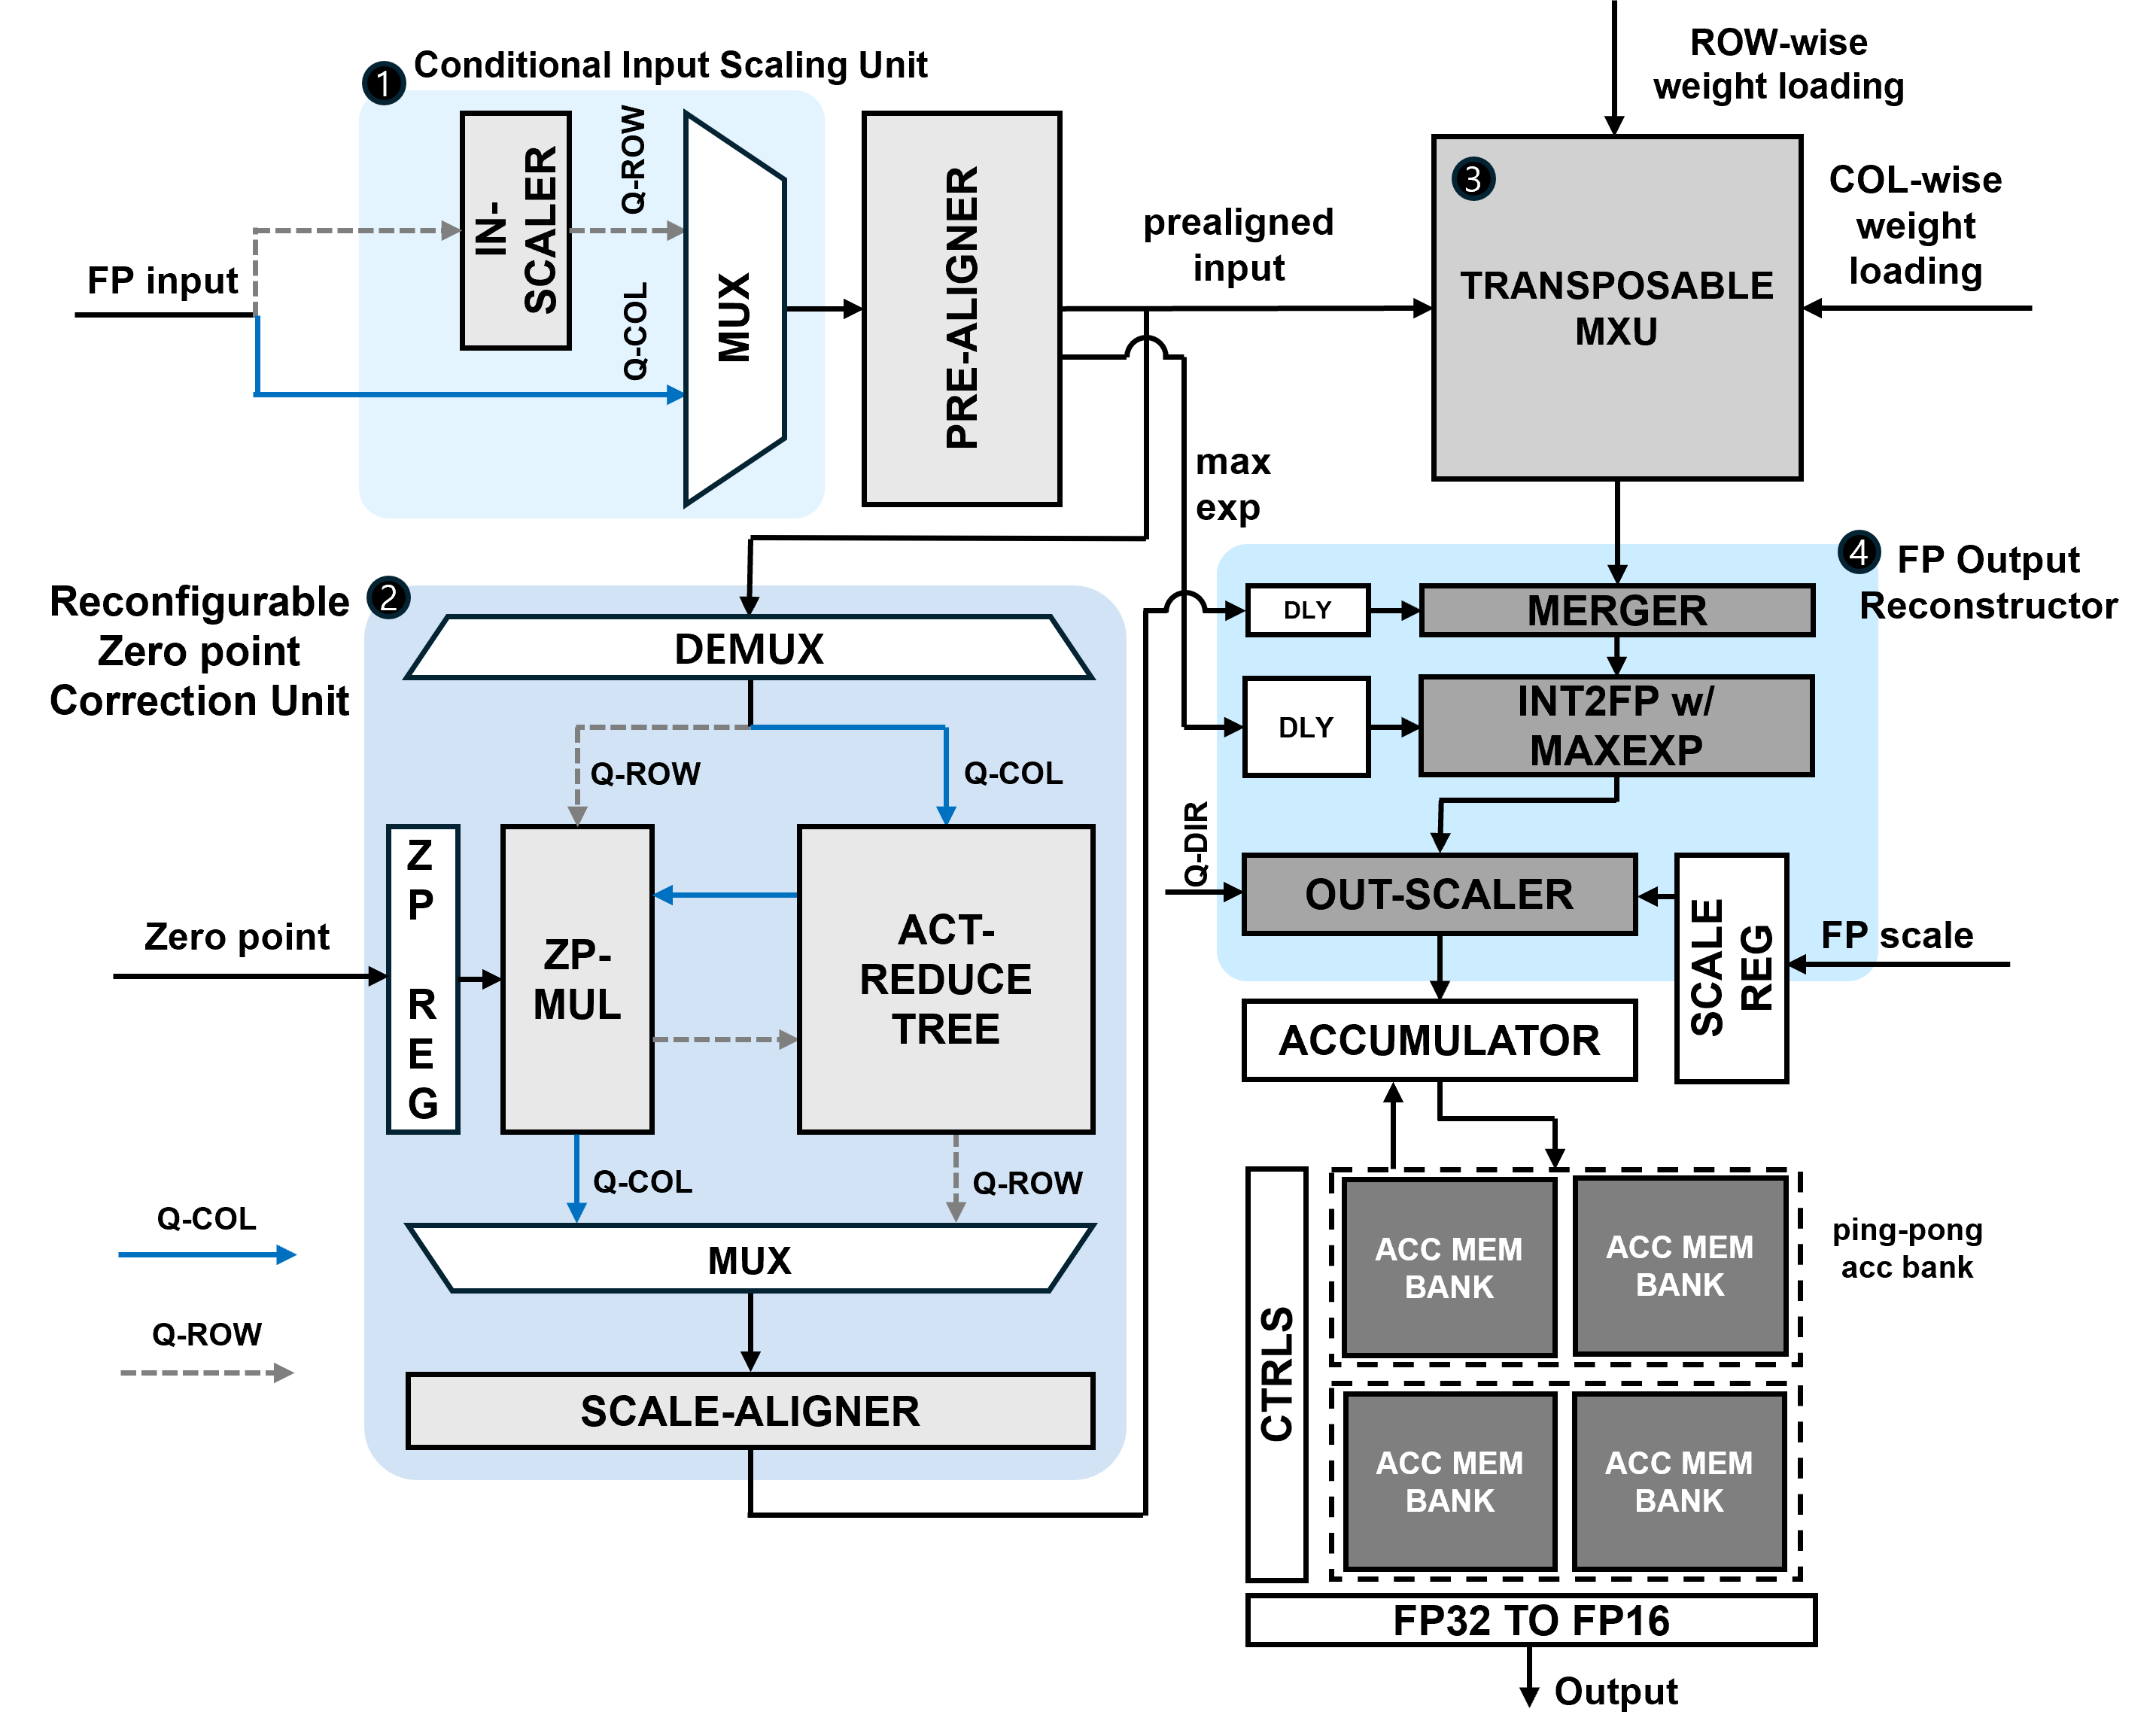
\includegraphics[width=0.62\linewidth]{figures/gemm_engine.png}
    \caption{RHS-axis-reconfigurable \fpint{} GEMM unit with scale-folding datapath and dual RHS load paths.}
    \label{fig:fpint-gemm-unit}
\end{figure}

%-------------------------------------------------------------
% flash attention은 일단 구현안하는 방향으로.. 일이 너무 많아지고 해서 얻을게 크게 없는듯
%-------------------------------------------------------------
%FIGNA SYSTEM programmable하기 때문에 Attention kernel을 FP-INT native한 FlashAttention-style로 구현할 수 있다 (Listing \ref{lst:fpint-flash-attn}).
%Q, K, V tile을 SRAM으로 가져오고, QK$^T$를 \fpint{} MXU에서 계산한다.
%이후 online softmax를 수행하고, softmax 결과와 quantized V 사이의 PV product도 \fpint{} MXU에서 처리한다.
%이 구조는 KV cache를 FP로 복원하지 않고도 attention 전체를 실행하는 것을 목표로 한다.

%\begin{lstlisting}[caption={FPINT naive flash attention.}, label={lst:fpint-flash-attn}]
%# TODO: replace this with code or pseudo-code
%for i in range(N):
%    y[i] = compute(x[i])
%\end{lstlisting}

이 설계의 핵심 효과는 quantized attention에서 FP fallback을 제거하는 것이다.
Linear layer만 \fpint{}로 가속하면 long-context workload에서 attention이 새로운 bottleneck으로 남는다.
반면 제안하는 MXU는 QK$^T$와 PV를 모두 native \fpint{} GEMM으로 실행할 수 있으므로, \wkv{} quantized model의 주요 GEMM path를 linear layer부터 attention layer까지 end-to-end로 가속한다.

\section[Memory System for Sustained FP-INT Utilization]{Memory System for Sustained \fpint{} Utilization}
\label{sec:memory-system}

\fpint{} MXU는 FP$\times$FP Tensor Core보다 작은 area와 낮은 energy로 더 많은 MAC을 제공할 수 있다.
그러나 MAC density의 증가는 곧 operand bandwidth demand의 증가를 의미한다.
기존 GPU-style datapath처럼 register file, shared memory, cache를 통해 모든 operand를 공급하면, port 수와 bank 수가 증가할수록 crossbar, arbitration, routing cost가 빠르게 커진다.
따라서 \ours{}의 memory system은 \fpint{} array를 단순히 core 옆에 붙이는 것이 아니라, array가 요구하는 regular tensor traffic을 general-purpose memory path에서 분리하는 방향으로 설계한다.

\paragraph{Decoupled GEMM Execution}

제안하는 \fpint{} MXU는 SIMT register file과 tightly coupled된 tensor instruction으로 동작하지 않는다.
SIMT kernel은 warp specialized 방식으로 GEMM 연산에 필요한 정보를 지정된 MMIO space에서 write하고 doorbell register에 write하는 방식으로 request를 issue한다.
GEMM CMD의 issue가 성공하면 gemm engine 내부의 micro-op generation FSM이 descriptor를 tile-level sequence로 확장하고, DMA와 local DMA는 그 명령어를 받아 HBM에서 TMEM으로 TMEM에서 GEMM engine으로 데이터를 옮긴다.
이 구조는 큰 MXU를 register file bandwidth와 warp operand scheduling에 묶어두지 않고 simple한 interconnection fabric 덕분에 low cost로 bandwidth를 충분히 유지할 수 있다.
SIMT pipeline은 launch, synchronization, non-GEMM vector operation을 담당하고, GEMM engine은 long-running tensor operation을 독립적으로 진행한다.

\paragraph{Partitioned On-Chip Tensor Storage}

Local memory는 기존 load/store, inter-thread communication, scalar/vector kernel을 위해 flexible access를 유지해야 한다.
반면 GEMM operand stream은 tile shape와 access order가 정해져 있으므로 full flexibility보다 banked bandwidth가 중요하다.
\ours{}는 on-chip SRAM을 general-purpose local memory와 MXU 전용 tensor memory와 accumulator memory로 분리한다.
Tensor memory와 accumulator memory는 restricted access pattern을 전제로 bank 수와 data width를 확장하고, local memory는 기존 SIMT programming model을 유지한다.
또한 partial sum은 operand보다 bitwidth가 크고 access pattern도 다르기 때문에 gemm engine 내부의 별도의 accumulator memory에 저장한다.
이 분리는 input/weight bandwidth와 partial-sum read-modify-write traffic이 서로 간섭하지 않게 하며, deeply pipelined 된 GEMM datapath에서 valid-ready protocol에서 ready signal을 없앨 수 있어서 control로 인한 overhead를 최소화 시킬 수 있다.

\paragraph{Direct-Connected Tensor Data Path}

HBM pseudo-channel과 tensor memory bank를 fully connected crossbar로 연결하면 bandwidth는 유연하게 사용할 수 있지만, area와 routing overhead가 bandwidth에 비례하지 않고 더 빠르게 증가한다.
Figure \ref{fig:memory-system}는 HBM과 TMEM bank의 data width가 64 byte이고, PC 개수와 TMEM bank 개수가 8이며, input precision이 FP16인 경우의 memory subsystem이다.
여기서 $R_{\mathrm{MXU}}$는 MXU의 row dimension size로, GEMM engine이 한 input slice에서 consume하는 reduction-lane 개수를 의미하며 Figure \ref{fig:memory-system}에서는 32이다
\ours{}의 memory subsystem은 HBM--TMEM, TMEM--MXU 사이를 1:1 또는 interleaved mapping으로 연결하여 all-to-all fabric을 제거한다. 여기서 interleaved 방식은 예를 들어서 src port 4개와 dst port 8개를 연결할 때 destination port i는 source port i\%4와 연결되는 방식이다. \todo{Comment : 여기서 src port 개수가 dst port 개수보다 적은 상황이 맞나요? 반대여야 모듈로 4가 의미있는거 아닌가요?}
이 path는 hardware cost를 낮추는 대신 source와 destination address 사이에 bank mapping constraint를 만든다.
예를 들어 HBM PC와 TMEM bank의 data width가 DW byte이고 PC의 개수가 $NUM_{pc}$이고 TMEM bank의 개수가 $NUM_{tmem}$일 때 다음과 같은 alignment를 만족해야 한다.
\begin{equation}
    \mathrm{Addr}_{\mathrm{HBM}}
    \equiv
    \mathrm{Addr}_{\mathrm{TMEM}}
    \pmod{DW \cdot \min\left(\mathrm{NUM}_{pc}, \mathrm{NUM}_{tmem}\right)} .
    \label{eq:hbm_tmem_addr_constr}
\end{equation}

TMEM과 GEMM engine 사이에서는 GEMM engine이 한 번에 consume하는 tensor slice 단위로 base address constraint가 발생한다.
예를 들어, \ours{}의 GEMM engine은 input slice
$I[m, R_{\mathrm{MXU}} k : R_{\mathrm{MXU}}(k+1)-1]$를 읽어 내부 MXU에 공급한다.
이때 해당 slice의 첫 번째 원소인 $I[m, R_{\mathrm{MXU}} k]$는 항상 GEMM engine input port의 least-significant lane에 align되어야 한다.
이를 보장하기 위해, 해당 원소가 저장될 수 있는 TMEM address를 제한함으로써 TMEM과 GEMM engine 사이의 interconnect를 단순화한다.
따라서 GEMM engine이 consume하는 각 slice의 base address는 다음 alignment constraint를 만족해야 한다. \todo{Comment : R\_MXU 가 뭔지 언급해줘야 할 것 같아요.}
\begin{equation}
    \operatorname{Addr}_{\mathrm{TMEM}}
    \left(I\left[m, R_{\mathrm{MXU}} k\right]\right)
    \equiv
    0
    \pmod{
        \operatorname{lcm}
        \left(
            \operatorname{sizeof}(I) \cdot R_{\mathrm{MXU}},
            DW
        \right)
    } .
\end{equation}

이 제약은 arbitrary memory copy에는 불편하지만, GEMM tile movement처럼 regular한 tensor traffic에서는 software layout transform과 memory allocation의 간단한 확장으로 쉽게 만족시킬 수 있다.

\paragraph{Cache-Bypassed Tensor DMA}

Tensor traffic은 cache hierarchy도 우회한다.
Cache를 경유하면 HBM에서 cache bank, local memory, SIMT load/store path로 이어지는 general-purpose routing을 지나야 하고, 이 path를 \fpint{} MXU의 operand bandwidth에 맞춰 확장하면 다시 xbar와 multi-bank arbitration cost가 병목이 된다.
따라서 \ours{}는 tensor DMA가 HBM pseudo-channel에서 tensor memory bank로 직접 데이터를 이동하도록 한다.
이 선택은 cache pollution과 SIMT memory traffic과의 port conflict를 줄이고, tensor path를 simple interconnect로 scaling할 수 있게 한다.
대신 cache-bypassed path는 coherent cache protocol 밖에서 동작하므로, hardware가 자동으로 SIMT cache state와 tensor memory movement의 coherence를 보장하지 않는다.
Section \ref{sec:runtime-section}에서 설명하듯이 \ours{}는 이 문제를 GEMM kernel의 explicit synchronization으로 처리한다.

\begin{figure}[H]
    \centering
    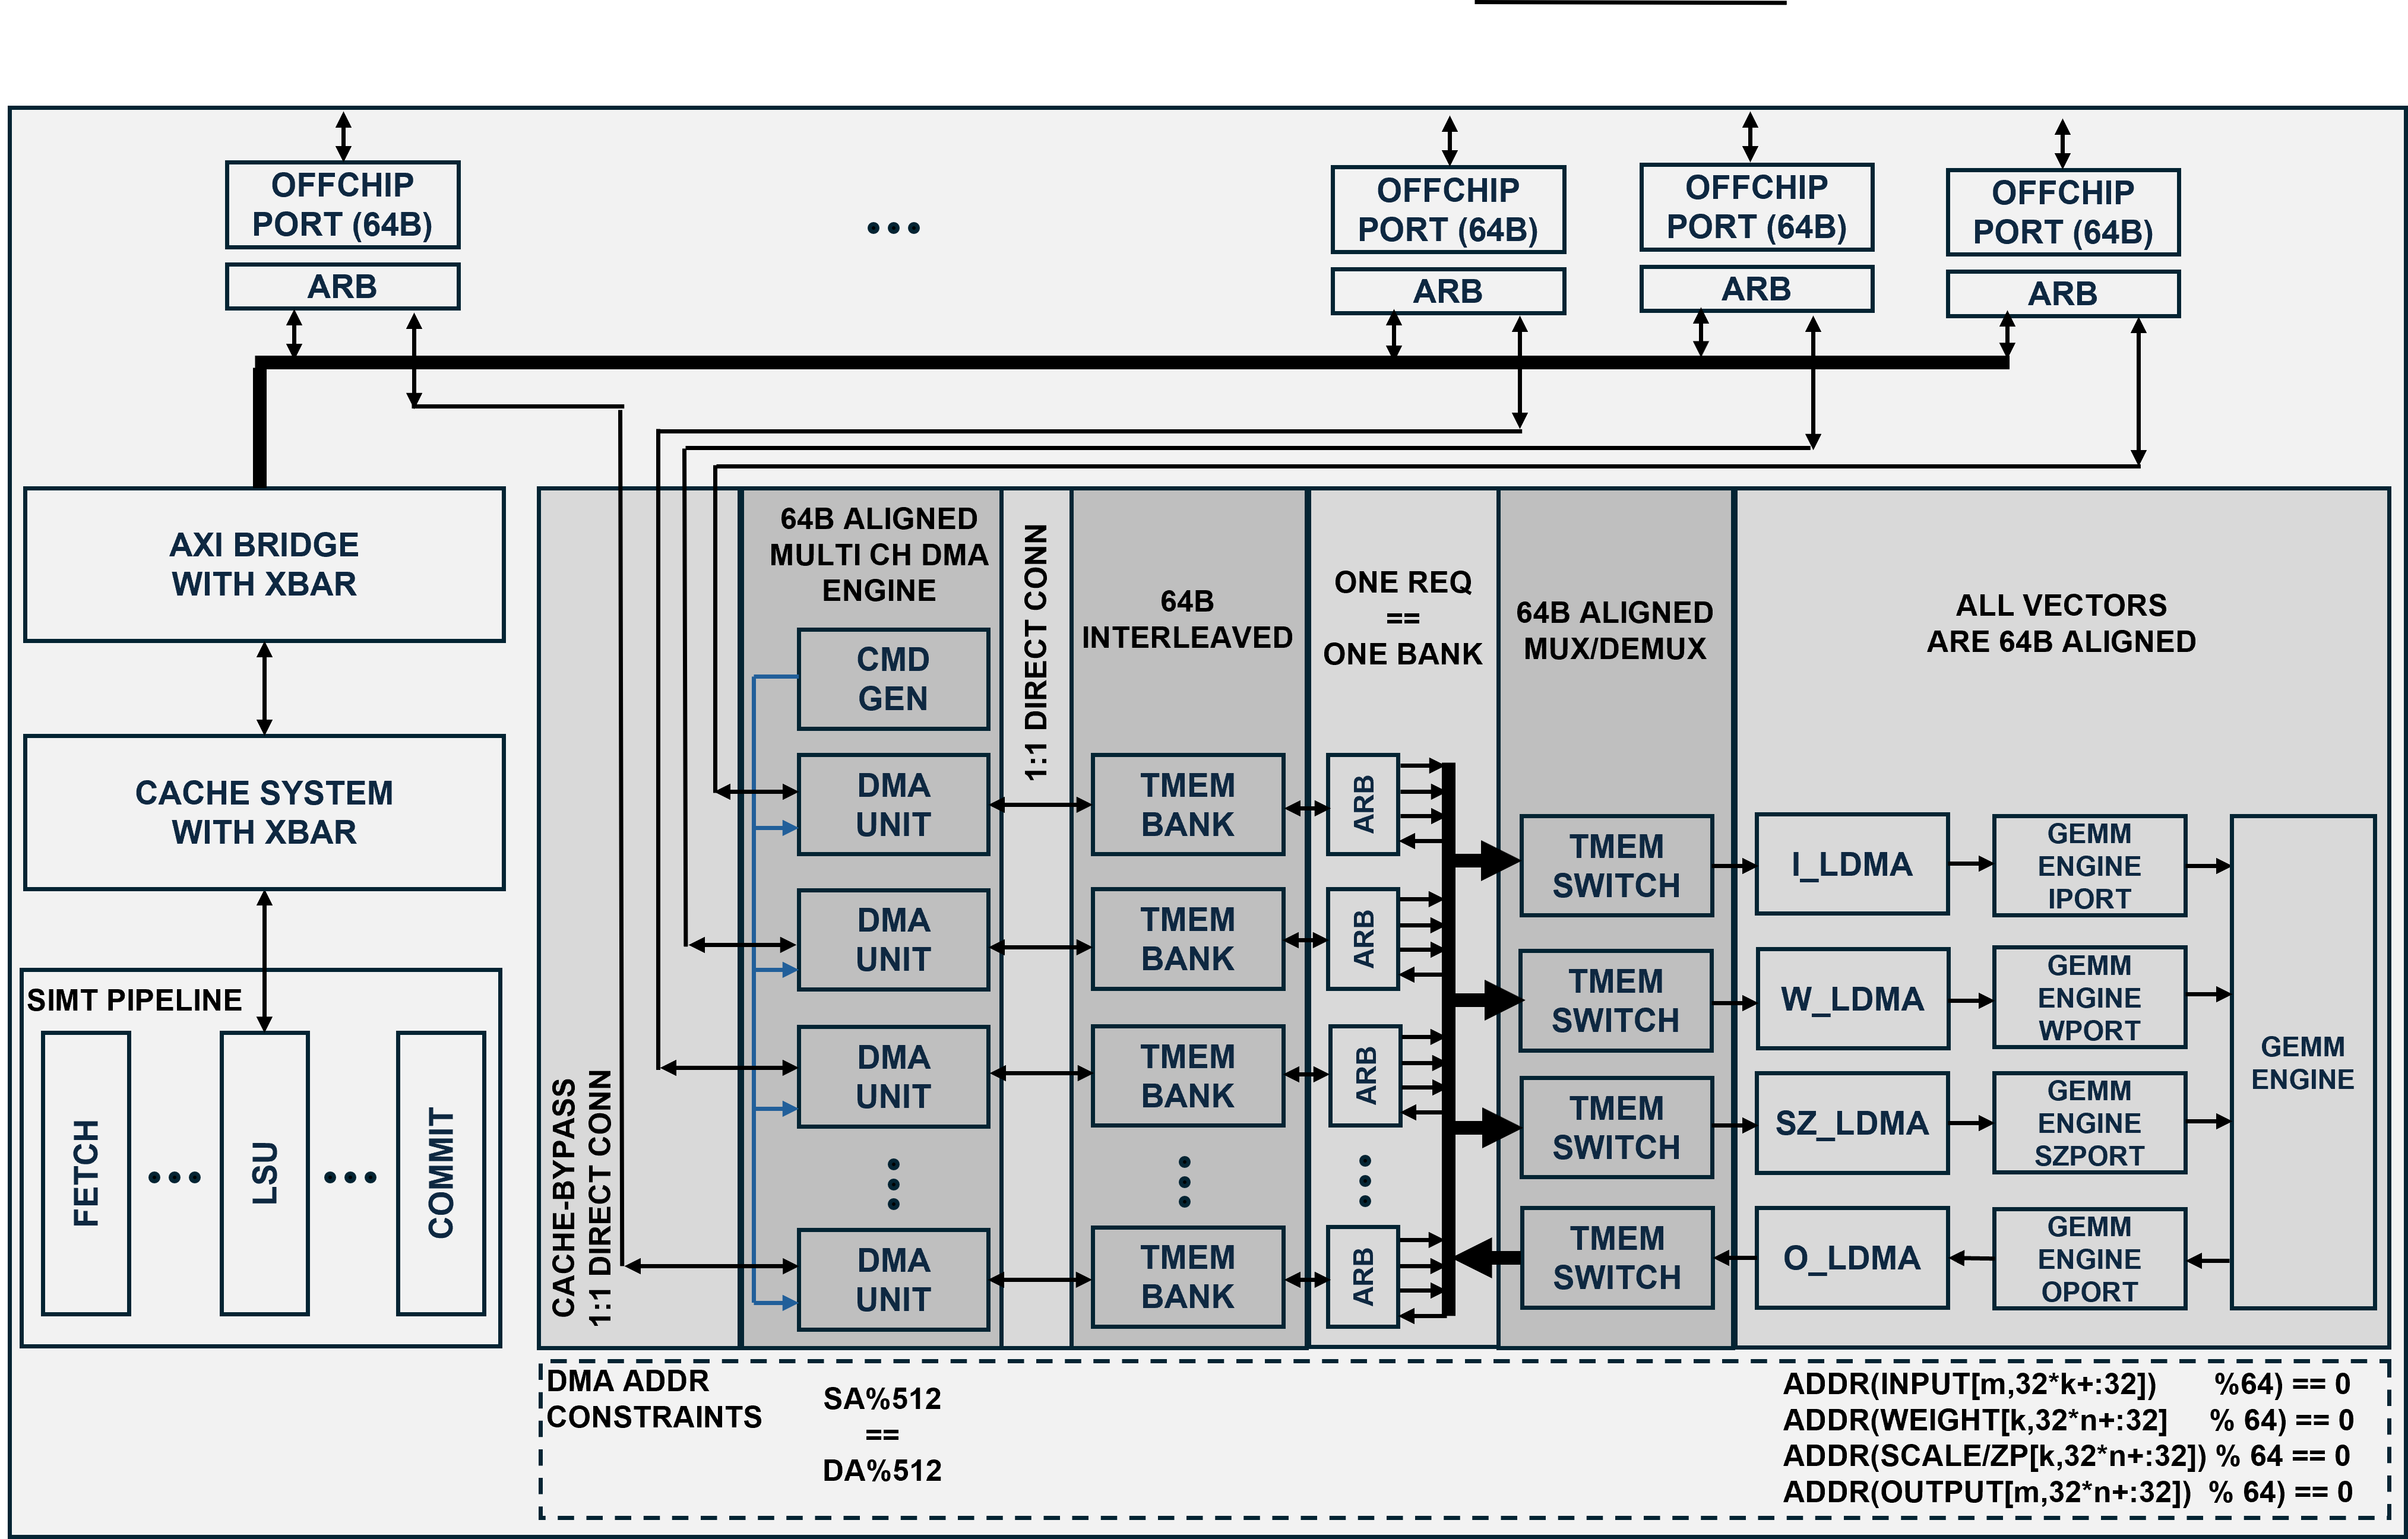
\includegraphics[width=0.62\linewidth]{figures/mem_sub_system.png}
    \caption{Memory system for sustaining large \fpint{} arrays with direct tensor data movement. \todo{Comment : CMD GEN이랑 DMA UNIT 들 있는 부분의 화살표가 겹쳐서 어디서 어디로 가는지가 명확히 안 보여요.}}
    \label{fig:memory-system}
\end{figure}

결과적으로 제안하는 memory system은 \fpint{} unit의 array-level efficiency를 operand supply 병목으로 잃지 않도록 한다.
Descriptor-driven GEMM execution, partitioned tensor storage, direct-connected DMA path, cache bypass를 함께 사용하여 general-purpose flexibility가 필요한 traffic과 high-bandwidth tensor traffic을 분리한다.

\section{Layout transformation and runtime extension}
\label{sec:runtime-section}

앞 절의 memory system은 hardware fabric을 단순화하는 대신 address alignment, bank mapping, non-coherent DMA라는 software-visible constraint를 만든다.
\ours{}의 software layer는 이 제약을 gemm의 규칙저인 tile access를 exploit해서 fused tile-major layout transform과 align-ware memory allocation으로 쉽게 만족시킨다.
핵심은 hardware가 복잡한 interconnection을 사용하지 않는 대신에, software가 tensor layout과 tensor가 memory에 저장되는 위치를 hardware가 가장 잘 소비할 수 있는 형태로 유지하는 것이다.

\paragraph{Tile-major Layout and Aligned Allocation}

\ours{} Section \ref{sec:memory-system}의 constraint를 tensor의 layout을 tile-major하게 바꾸고, tile size를 적절히 조절하면서 동시에 그 tile이 memory 상에 저장될 base address를 allocation할 때 같이 조절해서 쉽게 met한다.

\ours{}는 layout transform kernel을 SIMT에서 launch해서 GEMM의 input과 output tensor를 tile-major format으로 바꾼다. gemm 연산을 할 때 HBM에서 TMEM으로 옮기는 tile은 MT, KT, NT로 tile size가 정해지고 TMEM에서 gemm engine으로 오가는 tile은 $MT_{mxu}$, $KT_{mxu}$, $NT_{mxu}$로 정해진다. 이때 tile size를 section \ref{sec:memory-system}에서 말한 constraint의 modulus의 배수로 잡고, tile 안에 있는 원소들을 contiguous하게 저장해서 constraint가 쉽게 만족되도록 한다.

\ours{}는 vortex의 runtime을 확장해서 memory allocation을 할 때 기존의 requested size의 대한 align option 뿐 아니라 base address의 alignment도 제약으로 줄 수 있도록 한다.
그래서 runtime은 HBM allocation과 tensor memory allocation에 alignment constraint를 함께 적용해서 Eq. \ref{eq:hbm_tmem_addr_constr}을 만족시킨다.
Kernel은 임의 pointer를 DMA engine에 넘기는 대신, runtime이 보장한 aligned tensor object와 tile descriptor를 사용한다.
이 contract 덕분에 DMA는 wide barrel shifter나 general crossbar 없이 aligned burst만 처리하면 되고, allocation 단계에서 constraint를 한 번 해결한 뒤에는 tile-major layout와 적절한 tile size를 가지고 있으면 자연스럽게 Eq. \ref{eq:hbm_tmem_addr_constr}이 계속 met된다.

Tile-major layout과 alignment는 interconnection을 simple하게 할 수 있는 원동력을 제공함과 동시에 DMA 자체의 효율 또한 크게 높여준다. DMA efficiency는 request 하나가 얼마나 큰 contiguous segment를 이동할 수 있는지에 크게 좌우된다.
Response latency가 긴 경우 작은 request가 반복되면 request 간 bubble이 생기고, theoretical bandwidth를 실제 throughput으로 전환하기 어렵다.
그래서 row-major나 col-major로 tile을 전송하게 되면 row 또는 col 사이에 bubble이 생기고 pipeline이 deep한 long latency path를 DMA가 거치는 경우 DMA의 효율이 급격히 떨어진다.
tile-major layout의 경우 DMA가 가져와야하는 data가 연속된 주소에 있기 때문에 한개의 cmd만으로 DMA operation을 끝낼 수 있다.
\ours{}의 dma engine은 내부에 여러개의 DMA unit이 있는데 이 DMA unit은 stride, bound 등 정보를 기반으로 주소를 자동생성해서 데이터를 옮긴다. dma engine은 descriptor를 받고 controller가 내부적으로 target tensor 영역을 쪼개서 각 dma unit에 할당하고 병렬적으로 tensor를 가져온다. 이때도 \ours{}은 간단한 interconnection과 channel-bank mapping 덕분에 controller와 dma engine 내부의 mux, demux 등 logic을 최소화할 수 있다.


\paragraph{Explicit Ownership and Synchronization}

Cache-bypassed DMA는 coherence 문제를 만든다.
그러나 \wkv{} GEMM kernel에서는 SIMT pipeline과 \fpint{} engine이 accumulation 중인 같은 tile을 동시에 arbitrary하게 접근하지 않는다.
각 tensor tile은 phase별 owner가 명확하다.
SIMT code 또는 runtime이 descriptor와 metadata를 준비하고, DMA가 HBM에서 tile을 tensor memory로 이동시키며, MXU가 tensor memory와 accumulator memory를 소비하고, SIMT pipeline은 accumulation이 끝난 이후에만 결과를 읽는다.
Ownership이 SIMT와 tensor path 사이에서 넘어가는 지점에는 kernel이 explicit fence 또는 synchronization을 삽입하여 visibility를 보장한다.
즉 \ours{}는 coherence를 복잡한 hardware로 해결하지 않고 tile level의 explicit synchronization으로 해결한다.

\paragraph{Fused Layout Transformation}

Layout transform을 독립 kernel로 실행하면 tensor path에서 얻은 이득을 별도의 memory pass가 상쇄할 수 있다.
\ours{}는 Q/K/V projection, quantization, GEMM preparation, output movement와 같은 주변 kernel에 layout transform을 fuse하여 transform cost를 숨긴다.
이 방식은 tensor가 HBM에 저장되는 순간부터 DMA-friendly layout을 유지하게 만들고, direct-connected path가 요구하는 alignment를 steady-state kernel execution 안에서 만족시킨다.

\begin{figure}[H]
    \centering
    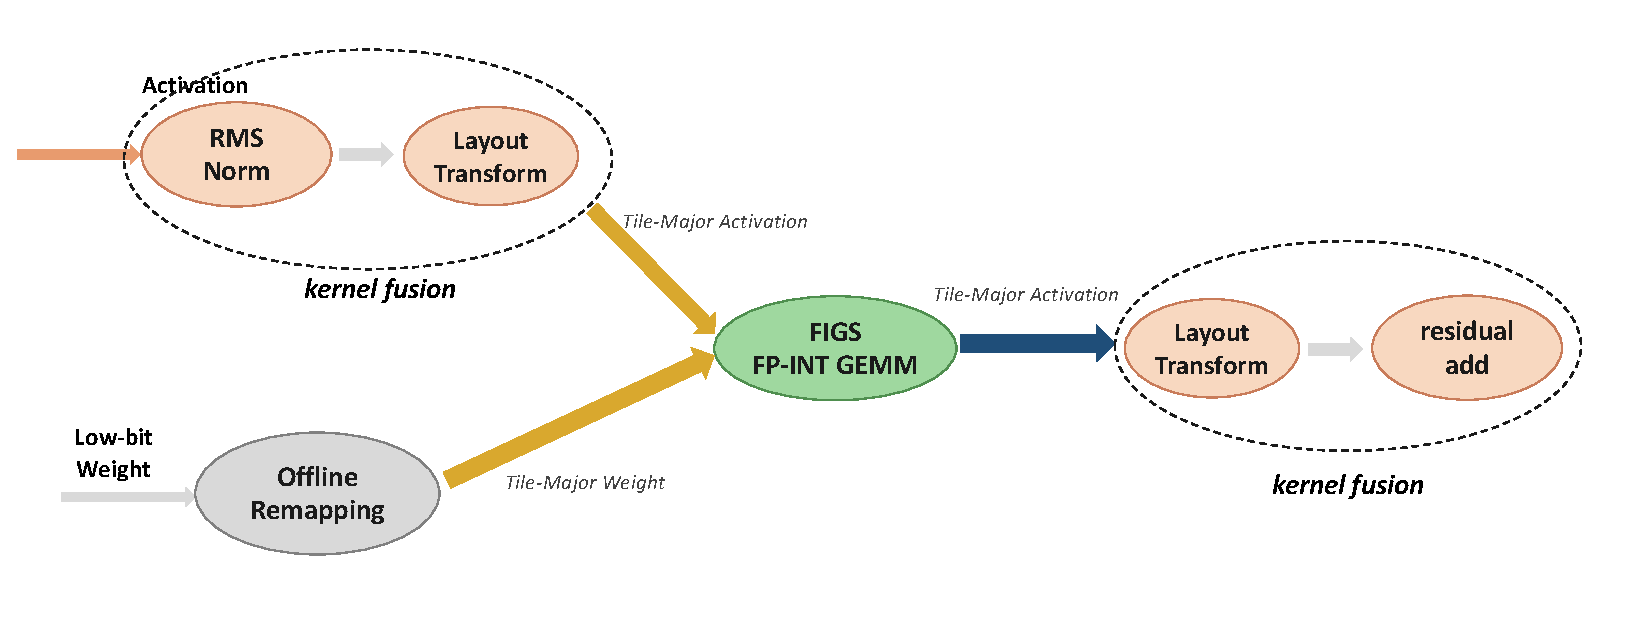
\includegraphics[width=0.92\linewidth]{figures/kernel_fusion.pdf}
    \caption{Fused layout transformation for feeding cache-bypassed tensor DMA.}
    \label{fig:fuse_layout_transform}
\end{figure}

%\section{End-to-End Stack Implementation}

%많은 accelerator 연구는 GEMM kernel 단독으로 실제 hardware가 아닌 simulator에서 array-level efficiency를 보인다.
%그러나 실제 LLM inference는 integration with frontend frameworks, runtime, programming model, non-GEMM operator등 이 함께 동작해야 한다.

%\paragraph{Runtime Abstractions for Tensor Memory}

%\ours{}는 Vortex runtime을 확장하여 tensor memory allocation, HBM alignment, scale/zero-point register management, GEMM descriptor setup과 doorbell launch primitive를 제공한다.
%Runtime은 앞 절의 address contract를 allocation API 안에 캡슐화하고, kernel은 aligned tensor object와 tile descriptor를 통해 DMA와 MXU를 제어한다.
%또한 cache-bypassed tensor path가 요구하는 synchronization primitive를 제공하여, kernel이 ownership transfer 지점에서 필요한 fence를 명시할 수 있게 한다.

%\paragraph{PyTorch Integration}

%PyTorch integration은 PrivateUse1 backend를 통해 quantized operator를 Vortex kernel로 dispatch한다.
%Frontend는 \wkv{} quantized tensor와 metadata를 유지하고, backend는 operator pattern에 따라 native \fpint{} linear, QK$^T$, PV kernel을 선택한다.
%이 stack 덕분에 \ours{}는 단순 GEMM microbenchmark가 아니라 실제 LLM inference graph 안에서 memory system, runtime layout, native attention support가 함께 작동하는지를 평가할 수 있다.

%\paragraph{Descriptor-Driven Kernel Organization}

%Kernel은 GEMM micro-op를 직접 생성하지 않는다.
%각 GEMM phase에서 SIMT code는 runtime이 준비한 tile descriptor를 읽고, MMIO register에 matrix shape, base address, stride, qdir, load direction, post-processing mode를 programming한 뒤 doorbell register를 write한다.
%GEMM engine은 request slot을 allocate하고, allocation이 성공한 request에 대해 내부 FSM을 시작한다.
%FSM은 descriptor로부터 반복적인 micro-op stream을 생성하여 aligned DMA movement, row/column RHS load, qdir-aware MXU execution, accumulator memory update, completion signaling을 순서대로 발행한다.
%Kernel은 completion을 polling 또는 wait primitive로 확인하고, cache-bypassed tensor path와 SIMT path 사이의 ownership이 넘어가는 지점에서 fence를 수행한다.
%이 구조는 software command queue 방식보다 command overhead를 크게 줄인다.
%기존 CMD queue 방식에서는 kernel이 bit field를 조립하고 store 명령으로 command를 enqueue해야 했는데, warp 하나가 생성할 수 있는 scalar command bandwidth가 큰 \fpint{} MXU를 feed하기에 부족했다.
%Descriptor-driven FSM은 per-micro-op command generation을 hardware sequencer로 옮겨, kernel이 micro-op 수에 비례하는 command stream이 아니라 $O(1)$ GEMM descriptor만 제출하도록 만든다.
%SIMT pipeline은 softmax, RoPE, layernorm, residual과 같은 non-GEMM operation도 같은 programming environment 안에서 처리하므로, unsupported operator가 CPU로 fallback하는 비용을 피할 수 있다.


\section{Evaluation}

\subsection{Setup}

\paragraph{Hardware Candidates}
본 논문은 네 가지 hardware candidate를 비교한다.

\paragraph{C1: \Cone{}}
Vortex에 FPxFP TCU를 enable해서 구현한다. C1은 모든 GEMM 연산을 int로 quantized 된 operand를 SIMT core로 dequantization 한 이후에 FP TCU로 실행한다.

\paragraph{C2: \Ctwo{}}
C1에서 decoupled \fpint{} mxu를 추가한다. QKV generation, FFN의 linear projection은 \fpint{} mxu로 처리하고 attention의 $QK^T$ 와 PV는 FP TCU로 처리한다. C2는 기존의 linear operation만 \fpint{}로 처리하는 FIGNA/FIGLUT/LUT-TC 를 대변한다. 

\paragraph{C3: \Cthr{}}
Both linear layers and attention QK$^T$/PV operations are executed on the \fpint{} MXU. The memory subsystem remains naive.

\paragraph{C4: \Cfou{}}
Final design with \fpint{} execution for both linear and attention kernels, together with memory subsystem, runtime, and layout optimizations.

Table \ref{tab:candidates}는 각 candidate의 parameter를 보여준다. 모든 candidate에 대해서 core는 1개를 사용하고 있고 warp의 갯수는 4개, warp 당 thread는 32개를 사용한다. TCU의 size는 thread 갯수에 따라서 8x4x4를 사용한다. \fpint{} gemm engine의 경우 32x32 array를 사용한다. Cache size는 모든 candidates에 대해서 동일하게 설정했고 local memory size도 동일하게 설정했다. tensor memory가 있는 경우에는 local memory와 tensor memory를 합친 size를 다른 candidates의 local memory랑 동일하게 설정했다. 

각 candidate는 같은 \wkv{} quantized model을 입력으로 사용하되, 어떤 연산을 어떤 hardware path로 실행하는지가 다르다.
면적은 28nm node에서 synopsys design compiler를 사용해서 100MHz target으로 합성 후 측정했다.
파워는 candidates를 FPGA에 100MHz를 target으로 PnR한 이후에 xrt-smi를 사용해서 kernel을 여러 번 돌리면서 board power를 측정했다. 이때 idle power를 측정된 power에서 빼서 dynamic power를 측정했다.

성능을 측정할 때는 면적 또는 power로 normalize해서 공정하게 평가한다.


\begin{table}[H]
\centering
\caption{Hardware candidates for ablation study.}
\label{tab:candidates}
\begin{tabular}{p{0.12\linewidth}p{0.25\linewidth}p{0.10\linewidth}p{0.10\linewidth}p{0.15\linewidth}p{0.15\linewidth}}
\toprule
Candidate & Name & Num Warps & Num Threads & FP TCU Size & \fpint{} MXU Size \\
\midrule
C1 & \Cone{} & 4 & 32 & 8x4x4 & --  \\
C2 & \Ctwo{} & 4 & 32 & 8x4x4 & 32x32 \\
C3 & \Cthr{} & 4 & 32 & -- & 32x32 \\
C4 & \Cfou{} & 4 & 32 & -- & 32x32 \\
\bottomrule
\end{tabular}
\end{table}

\paragraph{Workloads}

평가는 prefill, generation, end-to-end inference를 모두 포함한다.
model은 llama2-7b 위주로 평가하고 model은 SpinQuant로 Weight와 KV를 4bit으로 quantization 했다. quantization option은 SpinQuant의 default parameter를 사용했다.

\paragraph{Software Implementation}
kernel launch code는 vortex runtime을 사용해서 C++로 구현했다. Kernel 구현은 vortex native하게 C++ 를 사용해서 구현한다.
Vector operation의 경우 일반적인 GPU kernel 처럼 SPMD style로 구현했다.
Gemm operation의 경우 FP tcu를 사용하는 경우는 vortex가 제공하는 tcu를 사용하는 kernel을 사용했고 \fpint{} mxu를 사용하는 경우에는 MMIO를 사용하는 kernel를 구현했다. kernel에서 하는 일은 먼저 정해진 주소에 행렬의 size, RHS의 tranposed 여부와 quantization 방향을 write하고 gemm node를 invoke한다. 그 이후에는 MMIO로 노출한 status register를 polling 하면서 gemm operation이 끝나기를 기다린다.
구현한 kernel launch code와 kernel은 pytorch의 PrivateUse1 backend를 통해 deep learning frontend와 integration 하고 cuda를 사용하는 방식과 비슷하게 tensor를 .to method로 accelerator의 dram에 복사한 뒤에 pytorch operator를 call하는 방식으로 vortex kernel로 dispatch한다.
이 stack 덕분에 \ours{}는 단순 GEMM microbenchmark가 아니라 실제 LLM inference graph 안에서 memory system, runtime layout, native \fpint{} attention support가 함께 작동하는지를 평가할 수 있다.
%Prefill은 compute-bound 성격이 강하므로 native \fpint{} compute의 효과를 보기 좋다.
%Generation은 KV cache access와 attention path가 중요하므로 \fpint{} attention과 memory subsystem의 효과를 보기 좋다.
%End-to-end inference는 GEMM 이외의 overhead와 software stack 통합 효과를 함께 보여준다.

%\todo{모델 후보: Llama 계열, Qwen 계열 등. Hidden size, head 수, KV head 수, context length, batch size를 표로 정리한다.}

\subsection{E2E 성능 향상}

Figure \ref{fig:main_result}는 C1--C4에 대해서 llama2-7b를 E2E로 inference 했을 때의 area/power normalized performance를 보여준다.
prefill에서는 batch size 1에 seq length를 512에서 16k까지 바꾸면서 실험하고 decode에서는 batch size를 1, 8, 64로 바꾸면서 seq length는 512에서 16k까지 바꾸면서 실험했다.
prefill에서는 area 와 power normalized performance 둘 다 모든 test case에서  \ours{}가 baseline 대비 각각 평균 x배, x배 높다.
sequence length가 증가하면서 \ours{}의 성능향상이 줄어드는데 softmax의 latency가 O(N2)으로 증가하면서 gemm의 portion이 줄어들기 때문이다.
C1과 C2를 비교하면 몇몇 case는 C1이 좋고 몇몇 case는 C2가 좋다.
C2가 sequence length가 길어짐에 따라 C1하고 효율이 비슷해지는데 seq len이 길어질수록 attention이 dominate하는데 C2는 fp tcu를 이용해 attention을 처리하고 fpint linear projection에 사용한다. fp tcu와 fpint를 같이 가지고 있기 때문에 같은 area혹은 power budget내에서 baseline인 C1에 비해 효율이 떨어지게 된다. 그래서 linear만 \fpint{}로 지원하는 Lut tc, figna등은 long sequence 경우에 오히려 효율이 떨어진다는 점을 시사한다.
C3는 linear와 attentino 둘다 \fpint{}로 하기 떄문에 fp tcu에 의한 overhead를 없앨 수 있어서 모든(?! 하나는 아님. decode, bs64) 경우에 C2보다 좋다. 하지만 memory subsystem과 DMA가 최적화되지 않은 상태로 naive하게 integraion된 상태라서 \fpint{}의 utilization을 높게 유지하지는 못해서 C4에 비해 모든 경우에 낮은 성능을 보인다. 

decode에서도 모든 case에서 \Cfou{}가 가장 좋은데 area, power normalized performance가 각각 평균 x배, x배 좋다.
sequence length가 커지면 C4의 성능 향상이 더 커진다. 이유는 xxx이다.

Table \ref{tab:layout-transform-overhead}는 gemm의 input, output tensor를 gemm friendly하게 만들기 위해 사용된 layout transform kernel의 overhead를 보여준다.
layout transform을 독립적으로 하면 overhead가 x\%인데 gemm의 직전, 직후 kernel과 fusion하면 overhead가 x\%로 줄어서 overhead가 거의 없는 수준이 된다.

% \begin{figure}[H]
%     \centering
%     \fbox{\parbox{0.92\linewidth}{
%     \centering
%     \vspace{10mm}
%     \textbf{Effective TOPS/mm2, TOPS/W. TOPS=1/latency}\\
%     C1, C2, C3, C4의 prefill/generation stage end-to-end speedup을 bar graph로 표시한다.\\
%     수평 점선으로 array level 이득을 표시해주면 좋을듯함. \\
%     model : llama2, llama3 \\
%     batch size : 1,4,16,64,256 with seq_length 512 and 8k+\\
%     seq length : 512,1k,2k,8k+ with batch size 1 and 256\\
%     \vspace{10mm}
%     }}
%     \caption{Ablation study showing how each design component contributes to system-level speedup.}
%     \label{fig:gemm-speedup}
% \end{figure}
\begin{figure}[H]
    \centering
    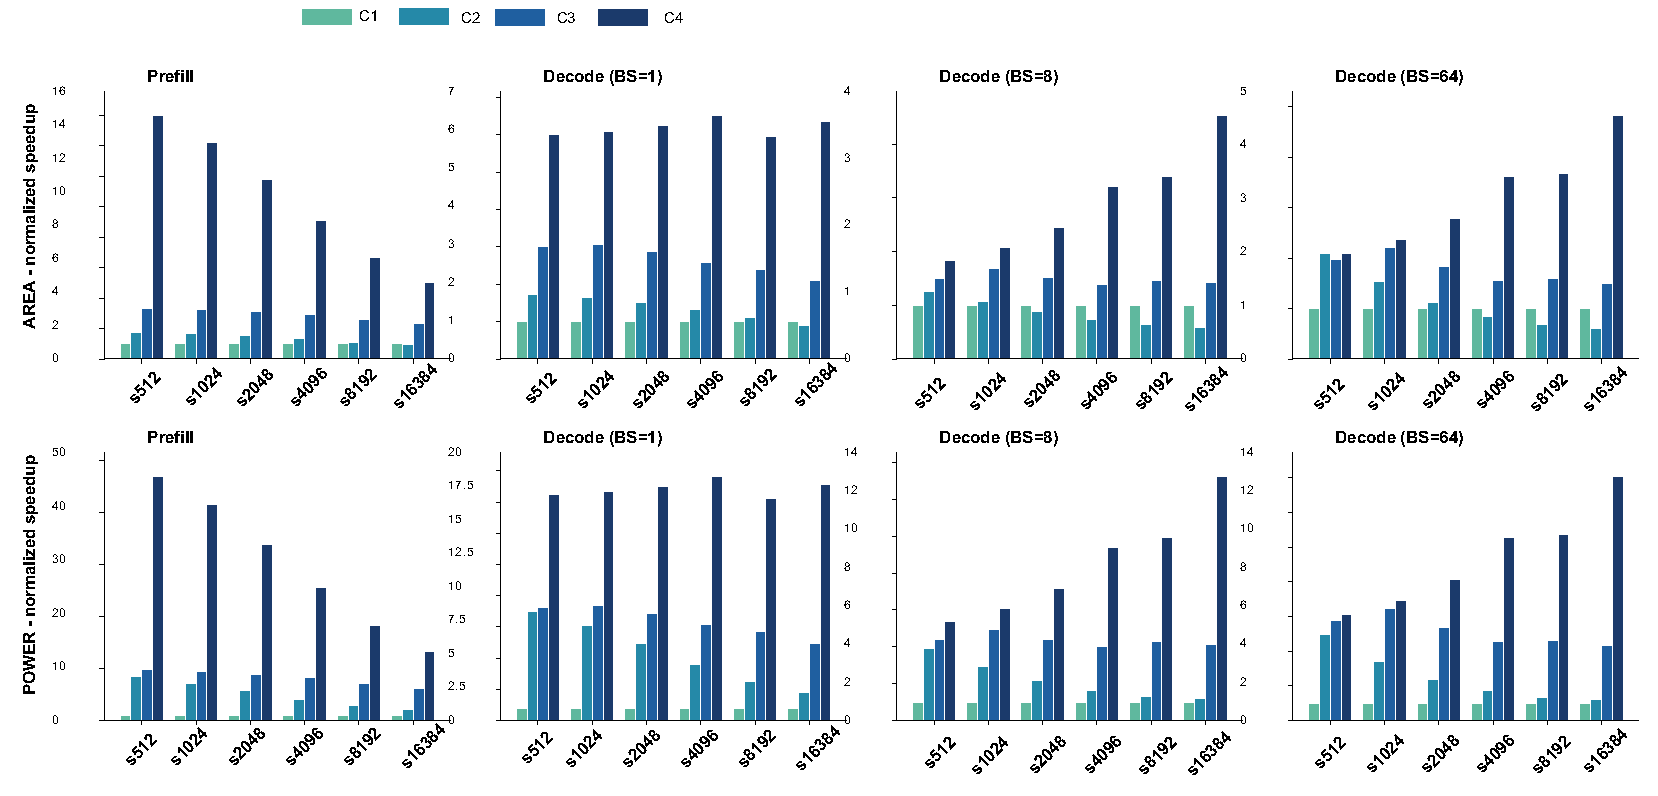
\includegraphics[width=0.92\linewidth]{figures/main_result_.pdf}
    \caption{element kernel 포함}
    \label{fig:main_result}
\end{figure}

%\begin{table}[H]
%\centering
%\caption{mxu util analysis. mxu util이 feeding 속도 따라가 같이 증가하는걸 숫자로 보여주자. kernel이 여러개니까 평균을 내야할듯함}
%\label{tab:memory-analysis}
%\begin{tabular}{p{0.32\linewidth}p{0.14\linewidth}p{0.14\linewidth}p{0.14\linewidth}p{0.14\linewidth}}
%\toprule
%Metric & C3 & C4 \\
%\midrule
%HBM bandwidth max/util &  \todo{측정} & \todo{측정} \\
%TMEM bandwidth max/util &  \todo{측정} & \todo{측정} \\
%MXU utilization & \todo{측정} & \todo{측정} \\
%\bottomrule
%\end{tabular}
%\end{table}

\begin{table}[H]
\centering
\caption{Overhead of fused layout transform is very low.}
\label{tab:layout-transform-overhead}
\begin{tabular}{p{0.32\linewidth}p{0.14\linewidth}p{0.14\linewidth}p{0.14\linewidth}p{0.14\linewidth}}
\toprule
kernel & plain kernel & after fusion & overhead(\%) \\
\midrule
rmsnorm &  {3745.2us} & {3750.46us} & {+0.1\%}\\
silu &  {16337.69us} & {16556.56us} & {+1.3\%}\\

\bottomrule
\end{tabular}
\end{table}

\subsection{성능 breakdown}

Figure \ref{fig:breakdown}은 linear projection과 attentino에 포함된 gemm 연산의 area/power normalized performance breakdown을 보여준다.

Figure \ref{fig:breakdown} 은 prefill과 decode 각각에 대해 short sequence(s512)와 long sequence(s16384)에서 linear projection(qkv\_proj, out\_proj, ffn)과 attention(qk, pv)에 포함된 GEMM 연산의 ISO-AREA 및 ISO-POWER normalized latency를 C1–C4로 분해하여 보여준다. 이 breakdown의 목적은 Figure \ref{fig:main_result}의 end-to-end speedup이 어떤 연산 path에서 발생하는지, 그리고 어떤 candidate가 어떤 bottleneck을 제거하는지를 분리하는 것이다.

모든 sequence length에서 linear projection(qkv\_proj, out\_proj, ffn)은 C1에서 C2로 넘어갈 때 큰 폭으로 감소한다. FP×INT MXU가 같은 면적에 더 많은 MAC을 제공하기 때문이다. 이 이득은 compute intensive한 영역인 prefill에서 두드러지는데, area-normalize할 경우 C2는 fp MAC과 fpint MAC을 동시에 가지고 있어 seq len이 클 때 baseline보다 좋지 않은 모습을 보인다. seq len이 커질수록 C2가 줄이지 못하는 영역인 attention(qk + pv) 연산이 커지기 때문이고 이는 그래프에서도 나타난다. 그러나 power-normalize의 경우 fp MAC과 fpint MAC을 동시에 가지고 있다고 하더라도 특정 timing에 한 path만 타게 되므로 C2가 baseline에 비해 나은 모습을 보인다. C3와 C4는 attention또한 fp-int path를 타기 때문에 모든 gemm path에서 baseline대비 훌륭한 모습을 보인다. 특히 long sequence에서 C2와도 큰 차이를 보이는 것을 볼 수 있다. 


% \begin{figure}[H]
%     \centering
%     \fbox{\parbox{0.92\linewidth}{
%     \centering
%     \vspace{10mm}
%     \textbf{E2E에서 area normalized latency + 각 kernel에서 소모한 power, enegy}\\
%     candidates : C1, C2, C3, C4. 수직 방향으로 쌓는다
%     model : llama2 \\
%     batch, seq length : (1, 512), (1, 8k+), (256, 512), (256, 8k+)
%     각 candidate의 kernel별 latency는 면적으로 normalize해서 수평 방향으로 stacked bar를 그린다. 이 때 수평방향 bar의 총 길이를 서로 다르게 냅두자. 그래야 C4가 더 빨리 끝나는게 티가난다. (즉 bar 길이를 전부 같게 normalize 하지 말자는 것) \\
%     power, energy는 각 kernel의 latency bar 밑에 tracing 한걸 그려준다. (FPGA board power 측정해서) \\
%     latency가 normalize 됐으니까 power도 같은 비율로 normalize 해준다. (latency가 짧아지면 power는 커져야함. energy는 바뀌는게 아니니까). board power는 그릴만할텐데 만약 DC로 측정한 power를 쓸 경우에 대해서는 평균 수평선 그리고 min,max를 std bar로 표현해두자 \\
    
%     \vspace{10mm}
%     }}
%     \caption{Kernel-level cycle breakdown for identifying bottlenecks.}
%     \label{fig:E2E}
% \end{figure}

\begin{figure}[H]
    \centering
    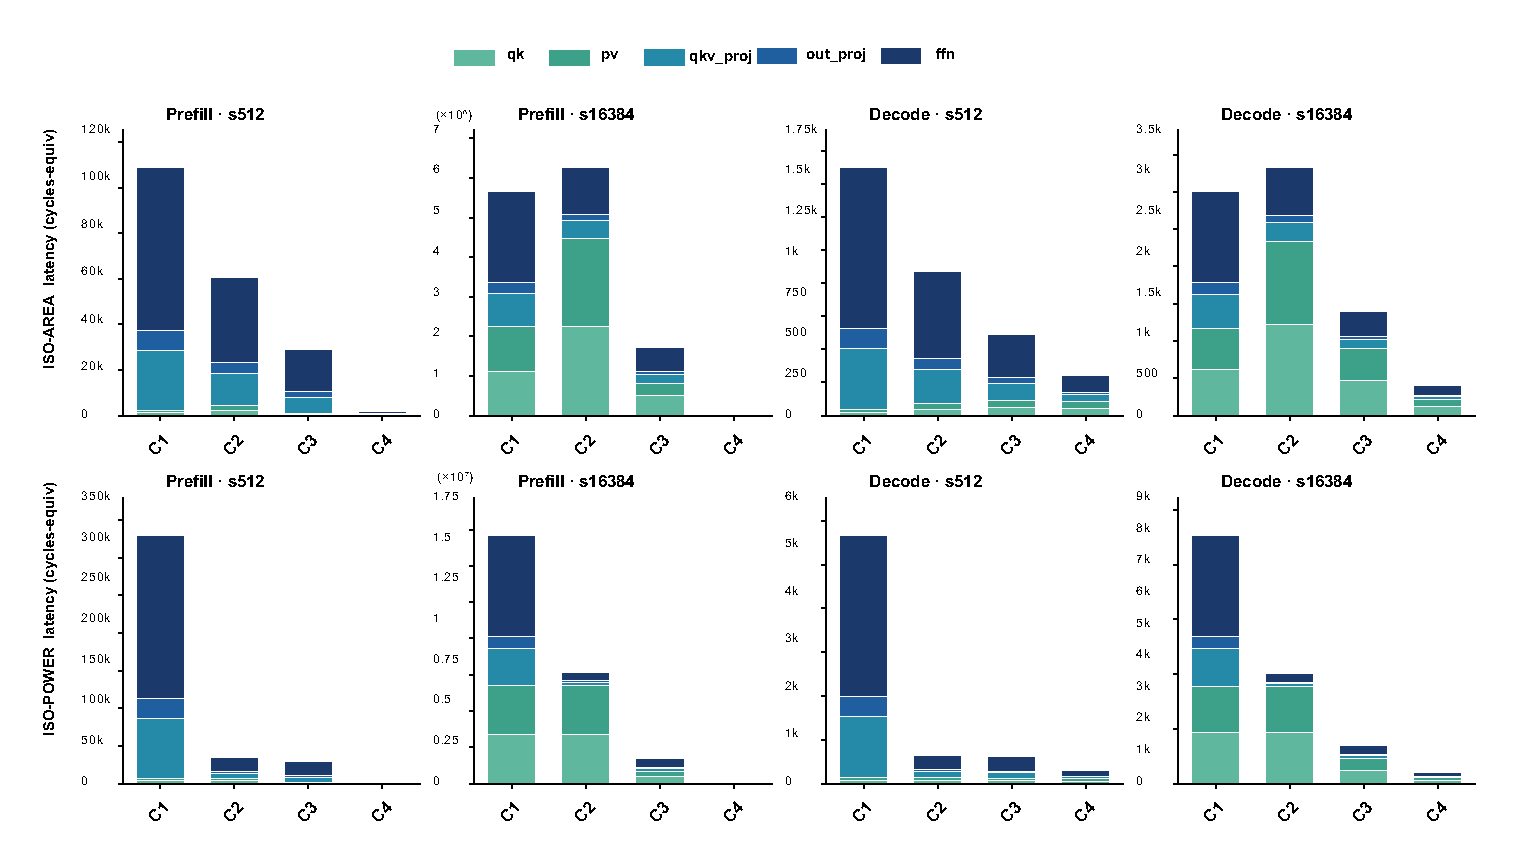
\includegraphics[width=0.92\linewidth]{figures/breakdown_result.pdf}
    \caption{element kernel 포함 x}
    \label{fig:breakdown}
\end{figure}


%\subsection{Comparison with Other Tensor Core Designs}
%WGMMA, Virgo와 비교 - 이 논문들에서 report하는 값인 1.6x와 2.85x를 사용, GEMM만 해당되고 GEMV는 report가 없기 때문 그리고  512 이상의 size gemm에서 저 값들이 유효하므로 seq len 512이상 prefill을 plot한다.

%\begin{figure}[H]
%    \centering
%    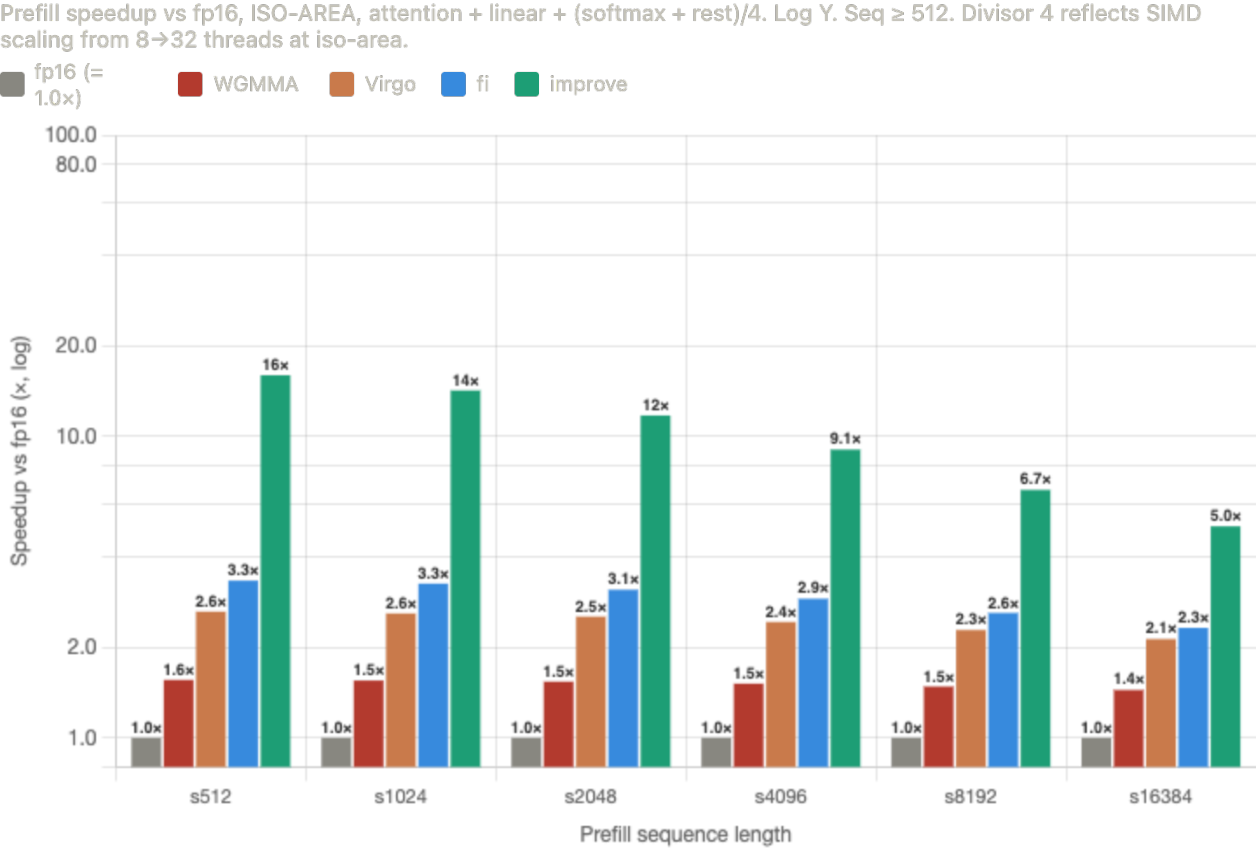
\includegraphics[width=0.92\linewidth]{figures/compare_prefill.pdf}
%    \caption{element kernel 포함}
%    \label{fig:wgmma_virgo}
%\end{figure}

\subsection{Accuracy}

% 다섯 번째 실험은 \wkv{} quantization이 model accuracy에 미치는 영향을 확인한다.
% 본 논문의 hardware는 quantized model의 연산을 효율적으로 실행하는 것이 목표이므로, 동일한 quantization algorithm을 사용했을 때 baseline GPU와 같은 numerical behavior를 유지해야 한다.
% Perplexity 또는 downstream task accuracy를 통해 accuracy degradation이 없거나 제한적임을 보인다. ()
이 실험은 WKV quantization이 model accuracy에 미치는 영향을 확인한다. 본 논문의 hardware는 quantized model의 연산을 효율적으로 실행하는 것이 목표이므로, 동일한 quantization algorithm을 사용했을 때 baseline과 동일한 numerical behavior를 유지해야 하며, hardware가 새로운 accuracy degradation을 유발해서는 안 된다.
Table \ref{tab:accuracy} 는 SpinQuant로 W4A16KV4 quantization을 적용한 Llama2-7B에 대해, FP×INT path를 적용하는 연산 범위를 달리한 네 가지 variant의 zero-shot accuracy를 비교한다. linear layer에만 적용한 경우(linear), attention의 $QK^T$/PV에만 적용한 경우(attn), 그리고 둘 다 적용한 경우(linear + attn)를 full WKV quantization(W4A16KV4)과 함께 보인다. 여덟 개 downstream task에 대한 평균 accuracy는 각각 63.10, 63.13, 63.01, 63.39로, 모든 variant가 0.4\%p 이내의 편차에 머문다. attention까지 FP×INT로 실행하는 본 논문의 target configuration(linear + attn)은 오히려 63.39로 가장 높은 평균을 보이며, ARC-c, ARC-e, BoolQ, HellaSwag 등 개별 task에서도 다른 variant 대비 일관되게 비슷하거나 더 나은 값을 유지한다.
이 결과는 FP×INT MXU가 linear와 attention path 모두에서 quantized operand를 native하게 처리하더라도 accuracy 손실을 일으키지 않음을 보여준다. 즉 본 논문이 제안하는 system-level 성능 향상은 numerical accuracy를 희생하지 않고 얻어진 것이며, quantization scheme에 의해 결정되는 accuracy와 hardware acceleration이 서로 독립적임을 확인한다.

\begin{table}[t]
\centering
\caption{Zero-shot accuracy and ppl comparison of W4A16KV4 variants.}
\label{tab:accuracy}
\resizebox{\linewidth}{!}{
\begin{tabular}{lccccccccc}
\toprule
\textbf{} & \textbf{ARC-c} & \textbf{ARC-e} & \textbf{BoolQ} & \textbf{HellaSwag} & \textbf{OpenBookQA} & \textbf{PIQA} & \textbf{SocialIQA} & \textbf{WinoGrande} & \textbf{Avg.} \\
\midrule
W4A16KV4 & 44.20 & 73.15 & 76.85 & 75.35 & 42.60 & 78.56 & 45.24 & 68.82 & 63.10 \\
W4A16KV4 (linear) & 44.37 & 72.98 & 76.24 & 75.34 & 43.20 & 78.40 & 45.29 & 69.22 & 63.13 \\
W4A16KV4 (attn) & 44.03 & 73.32 & 76.82 & 75.23 & 43.20 & 78.56 & 44.73 & 68.19 & 63.01 \\
\cellcolor{gray!12}{W4A16KV4 (linear + attn)} & \cellcolor{gray!12}{44.03} & \cellcolor{gray!12}{73.02} & \cellcolor{gray!12}{77.13} & \cellcolor{gray!12}{75.22} & \cellcolor{gray!12}{44.20} & \cellcolor{gray!12}{78.78} & \cellcolor{gray!12}{45.24} & \cellcolor{gray!12}{69.53} & \cellcolor{gray!12}{63.39} \\
\bottomrule
\end{tabular}
}
\end{table}


\subsection{breakdown and overhead analysis}
\paragraph{array level efficiency}
\fpint{} array가 FP$\times$FP TCU 대비 얼마나 높은 compute density와 energy efficiency를 제공하는지 측정한다.
FPxFP에 비해 x배 더 좋다. WoQ unit에 비해 overhead는 x로 매우 작다. Attention을 FPxINT로 할 수 있는 상황을 고려하면 WoQ gemm unit보다 WKV gemm unit의 효율이 effectively x배 좋다.(Figure \ref{fig:arr-level-break})

\begin{table}[H]
\centering
\caption{Relative array-level comparison. 28n tech. 100M. 32x32 size array}
\label{tab:array-level}
\begin{tabular}{p{0.22\linewidth}p{0.22\linewidth}p{0.22\linewidth}p{0.22\linewidth}}
\toprule
Unit & Precision & TOPS/mm$^2$ & TOPS/W \\
\midrule
FP TCU & FP$\times$FP & 1.0 & 1.0 \\
WoQ \fpint{} MXU & FP$\times$INT & 2.32 & 3.04 \\
WKV \fpint{} MXU & FP$\times$INT & 2.21 & 2.97 \\
\bottomrule
\end{tabular}
\end{table}

\begin{figure}[H]
    \centering
    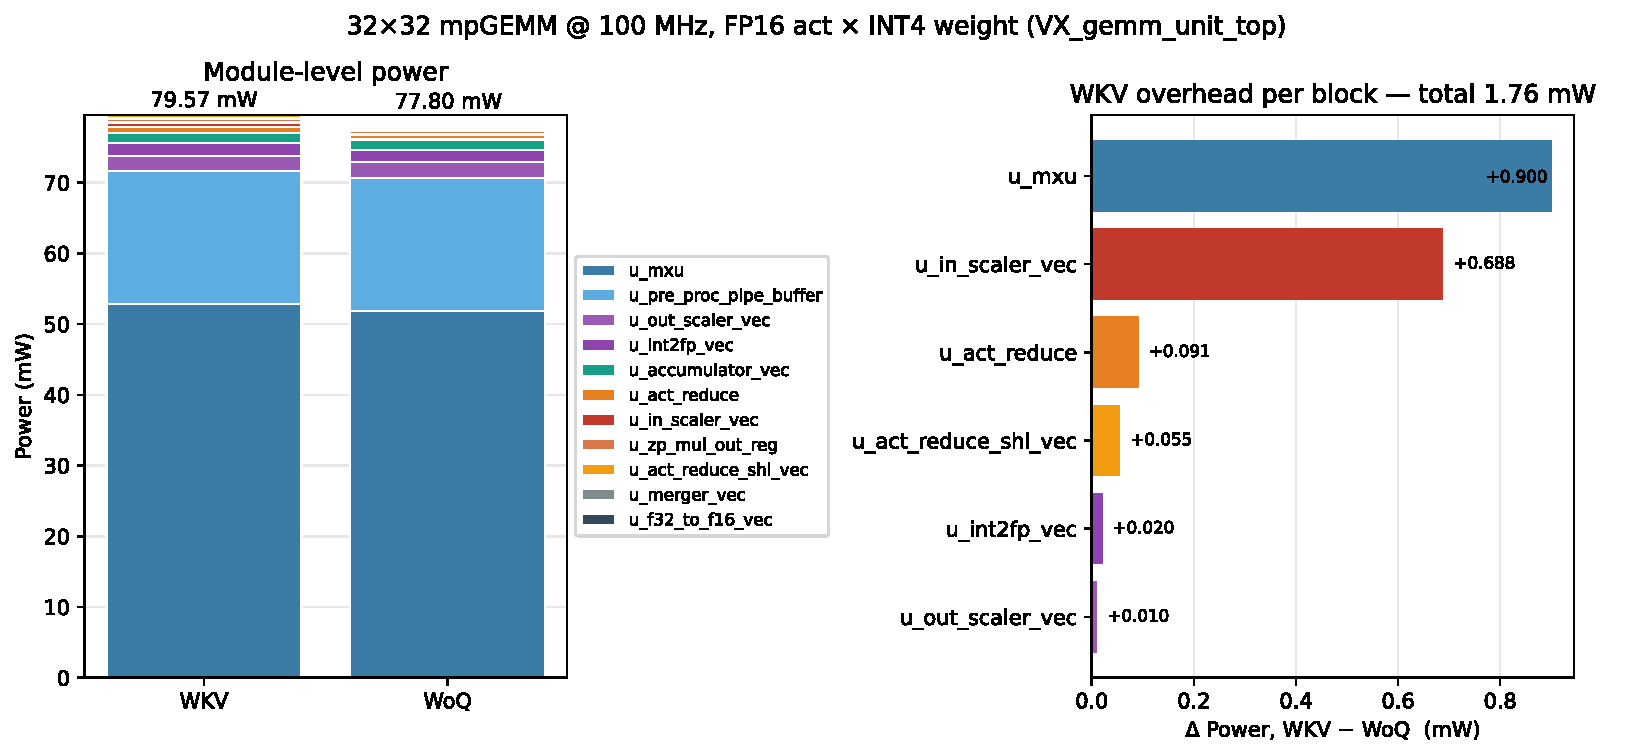
\includegraphics[width=0.92\linewidth]{figures/wkv_vs_woq_breakdown_refine.pdf}
    \caption{WoQ에 비해 WKV의 gemm unit level에서의 overhead가 작다는 것을 보여주자.}
    \label{fig:arr-level-break}
\end{figure}

\paragraph{area breakdown}
\ours{} 의 area breakdown 이다 (Figure \ref{fig:area-breakdown}). interconnection scaling 과 관련된 overhead 작다.
\begin{figure}[htbp]
    \centering
    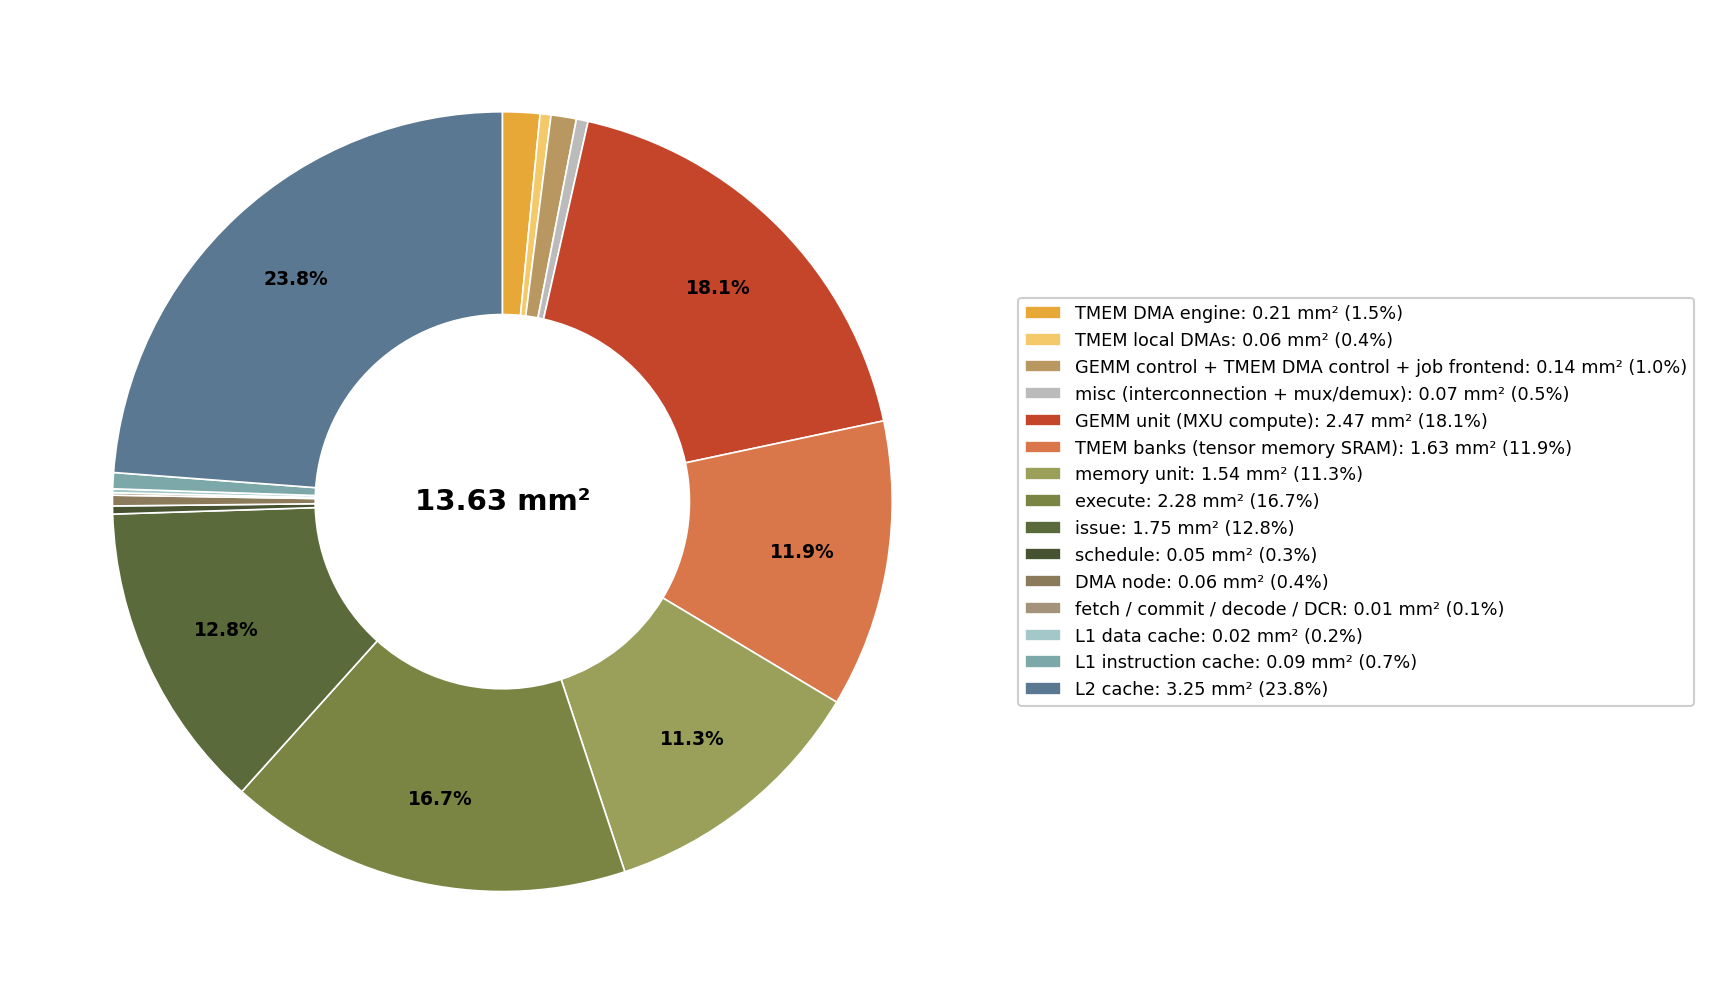
\includegraphics[width=0.92\linewidth]{figures/area_breakdown.png}
    \caption{simple interconnect 덕분에 dma와 interconnect 쪽에서 overhead가 거의 없다.}
    \label{fig:area-breakdown}
\end{figure}

%\paragraph{memory allocation}
%Padding overhead, HBM allocation fragmentation 작아서 layout optim한 것 문제 없다 (Table \ref{tab:alloc-overhead}).

%\begin{table}[H]
%\centering
%\caption{runtime padding and mem alloc overhead. llama2 inference할 때 각 kernel에서 overhead 측정}
%\label{tab:alloc-overhead}
%\begin{tabular}{p{0.28\linewidth}p{0.22\linewidth}p{0.22\linewidth}}
%\toprule
%kernel & Padding overhead & HBM allocation fragmentation \\
%\midrule
%qkv-gen & \todo{측정} & \todo{측정} \\
%qkt & \todo{측정} & \todo{측정} \\
%pv & \todo{측정} & \todo{측정} \\
%\bottomrule
%\end{tabular}
%\end{table}

%\subsection{Scalability}

%여섯 번째 실험은 core 수 또는 MXU 수를 늘렸을 때 성능이 확장되는지 확인한다.
%FPGA에 올라가지 않기 때문에 simx를 이용해서 실험한다.
%목표는 제안한 memory subsystem과 runtime이 single-core optimization에만 머무르지 않고 multi-core scaling에서도 병목을 만들지 않음을 보이는 것이다.(Figure \ref{fig:scale})
%\begin{figure}[H]
%    \centering
%    \fbox{\parbox{0.92\linewidth}{
%    \centering
%    \vspace{10mm}
%    \textbf{Scalability. Thput / mm2 으로 보여주자}\\
%    core의 크기 및 갯수를 늘리면서 성능 scaling 되는 것을 보여주자.\\
%    simx로 실험해야한다. 면적은 DC로 측정하자 \\
%    gemm만 보여주자.
%    core 갯수 : 1,2,4,8
%    array size : 32, 64, 128
%    model : llama2, llama3 \\
%    batch size : 1,4,16,64,256 with seq\_length 512 and 8k+\\
%    seq length : 512,1k,2k,8k+ with batch size 1 and 256\\
%    \vspace{10mm}
%    }}
%    \caption{Kernel-level cycle breakdown for identifying bottlenecks.}
%    \label{fig:scale}
%\end{figure}

\section{Conclusion}

\wkv{} quantized LLM inference는 memory footprint를 줄이는 것을 넘어, FP activation과 INT weight/KV 사이의 \fpint{} GEMM을 효율적으로 실행하는 문제로 바뀌고 있다.
기존 software-only approach는 dequantization을 잘 숨길 수 있지만 energy와 compute efficiency 측면에서 한계가 있다.
기존 hardware approach는 array-level 효율을 보였지만 attention, memory subsystem, programmable E2E execution을 충분히 다루지 않았다.
본 논문은 \fpint{} attention support, specialized memory subsystem, Vortex 기반 software/hardware stack을 함께 설계하여 \fpint{} unit의 array-level 이득을 실제 system-level LLM inference 성능으로 전환하는 것을 목표로 한다.

% -----------------------------------------------------------------------------
% References are intentionally left as TODOs in this Korean logic draft.
% Add BibTeX entries and replace the placeholders during the paper-writing phase.
% -----------------------------------------------------------------------------
\bibliographystyle{plain}
\bibliography{refs}

% this is git sync test b
% this is git sync test a

\end{document}
